% Created 2017-04-13 Thu 10:31
% Intended LaTeX compiler: pdflatex
\documentclass[10pt,aspectratio=1610]{beamer}
\usepackage[utf8]{inputenc}
\usepackage[T1]{fontenc}
\usepackage{graphicx}
\usepackage{grffile}
\usepackage{longtable}
\usepackage{wrapfig}
\usepackage{rotating}
\usepackage[normalem]{ulem}
\usepackage{amsmath}
\usepackage{textcomp}
\usepackage{amssymb}
\usepackage{capt-of}
\usepackage{hyperref}
\usepackage[english]{babel}\usepackage{etex}\usepackage{minted}\usemintedstyle{emacs}
\usepackage{tikz}\usepackage{amsmath}\usepackage[T1]{fontenc}\usepackage{lmodern}%\usepackage{arev}
\usepackage{booktabs}\usepackage[citestyle=alphabetic,bibstyle=authortitle]{biblatex}
\usepackage{pgfplots,pgfplotstable}\usetikzlibrary{pgfplots.groupplots}\usepackage[babel=true,kerning=true]{microtype}\usepackage{smartdiagram}
\addbibresource{class.bib}
\usetikzlibrary{mindmap,trees,shapes,arrows,spy,3d,decorations.pathmorphing,pgfplots.statistics,pgfplots.dateplot}
\pgfplotsset{compat=newest}
\hypersetup{colorlinks,linkcolor=,urlcolor=magenta}
\usetheme{DarkConsole}
\author{Mathieu Fauvel}
\date{\textit{[2017-04-26 Wed 13:30]--[2017-04-26 Wed 16:30]}}
\title{Classification of Hyperspectral Images}
\subtitle{GRSS Summer School}
\institute{UMR Dynafor}
\AtBeginSection[]{\begin{frame}<beamer>\frametitle{Outline}\tableofcontents[currentsection]\end{frame}}
\AtBeginSubsection[]{\begin{frame}<beamer>\frametitle{Outline}\tableofcontents[currentsubsection]\end{frame}}
\setbeamercovered{again covered={\opaqueness<1->{25}}}
\usefonttheme[onlymath]{serif}
\begin{document}

\maketitle
\begin{frame}{Outline}
\tableofcontents
\end{frame}

\section{Motivations}
\label{sec:org13dd03d}
\begin{frame}[label={sec:orgfced2c9}]{Classification of hyperspectral image is a challenging problem}
\begin{itemize}
\item Remember \emph{Introduction}: \alert{High dimensional data}
\begin{itemize}
\item High number of features
\item Large volume of pixels
\item Low number of labelled pixels
\end{itemize}
\item Practical issues:
\begin{itemize}
\item Intra-class spectral variability
\item Non-linear pre-processing (atmospheric/geometric corrections)
\item Noise in the data
\end{itemize}
\end{itemize}

\begin{center}
\begin{center}
\includegraphics[width=0.5 \linewidth]{./figures/hyper.png}
\end{center}
\end{center}
\end{frame}
\begin{frame}[label={sec:org93a833d}]{Classification overview}
\begin{columns}
\begin{column}{0.5\columnwidth}
\begin{itemize}
\item Reference data ?
\begin{itemize}
\item Supervised
\item Unsupervised
\item Semi-supervised
\end{itemize}
\item \(p(\mathbf{x},y)\sim\ ?\):
\begin{itemize}
\item Parametric models
\item Non parameterics models
\end{itemize}
\item Number of classes ?
\begin{itemize}
\item Multiclass
\item One-class / detection
\item Unknown
\end{itemize}
\end{itemize}
\end{column}
\begin{column}{0.5\columnwidth}
\begin{center}
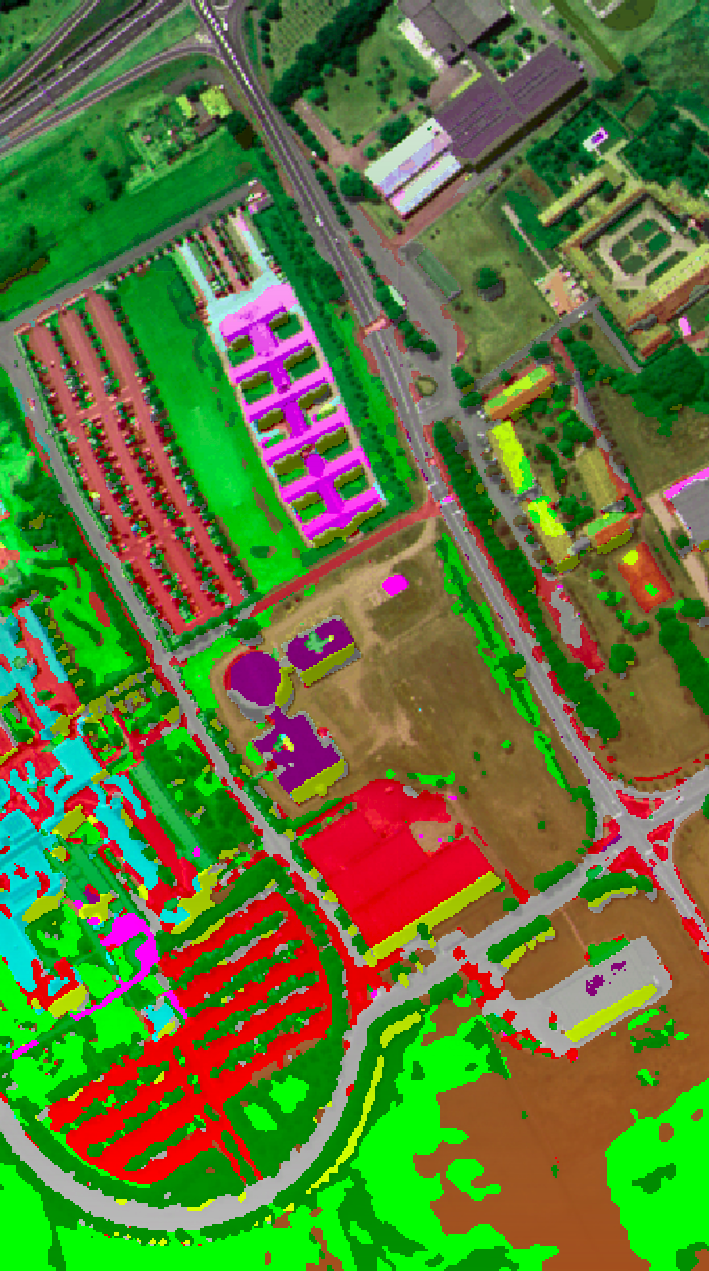
\includegraphics[width=0.55\textwidth]{./figures/uni.png}
\end{center}
\end{column}
\end{columns}
\end{frame}
\begin{frame}[label={sec:orge93ef81}]{Data sets used}
\begin{columns}
\begin{column}{0.5\columnwidth}
\begin{center}
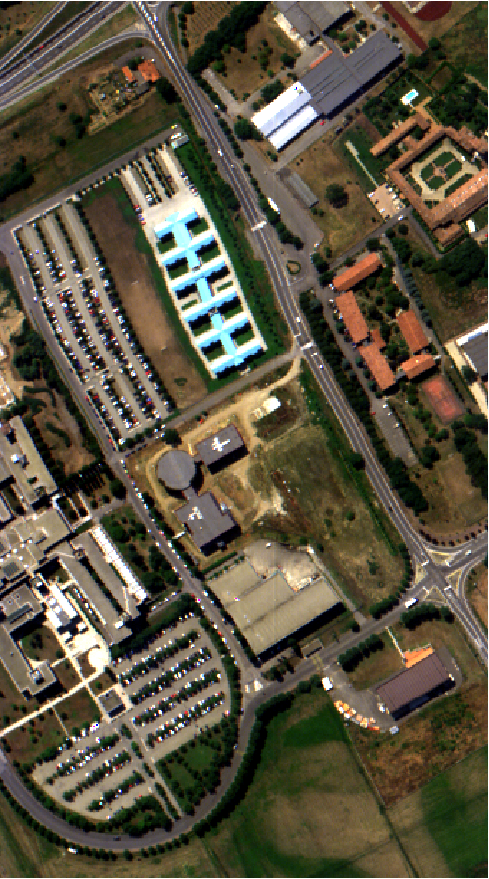
\includegraphics[width=0.55\textwidth]{./figures/university_color.png}
\end{center}
\end{column}
\begin{column}{0.5\columnwidth}
\begin{center}
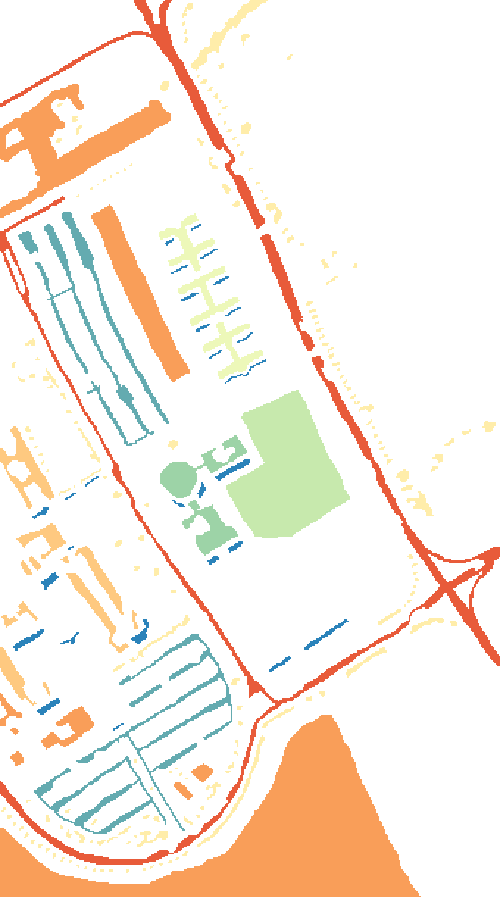
\includegraphics[width=0.55\textwidth]{./figures/university_gt.png}
\end{center}
\end{column}
\end{columns}
\end{frame}
\section{Introductory examples}
\label{sec:orga6ebf69}
\subsection{Influence of the number of samples}
\label{sec:org8bc32ed}
\begin{frame}[fragile,label={sec:org9e45da8}]{Experimental set-up}
 \begin{minted}[fontsize=\footnotesize,obeytabs=true,tabsize=4,bgcolor=bg]{python}
import scipy as sp
import rasterTools as rt
from sklearn.model_selection import train_test_split
from sklearn.discriminant_analysis import QuadraticDiscriminantAnalysis
from sklearn.metrics import f1_score

# Load data set
X,y=rt.get_samples_from_roi('../Data/university.tif','../Data/university_gt.tif')

# Split the data
X_, X_test, y_, y_test = train_test_split(X, y, train_size=0.50,random_state=0,stratify=y)

# Try differents size of the training set
SPLIT = sp.linspace(0.01,0.99,15)
F1,NS = sp.zeros_like(SPLIT),sp.zeros_like(SPLIT)
for i,split in enumerate(SPLIT):
    # Split the data
    X_train, _, y_train, _ = train_test_split(X_, y_, train_size=split,random_state=0,stratify=y_)
    # Learn the classifier
    clf = QuadraticDiscriminantAnalysis()
    clf.fit(X_train,y_train)
    # Predict the classes
    yp = clf.predict(X_test)
    #Compute the F1
    F1[i],NS[i] = f1_score(y_test,yp,average='weighted'),y_train.size
\end{minted}
\end{frame}

\begin{frame}[label={sec:org6194439}]{Results}
\begin{center}
  \begin{tikzpicture}
  \begin{semilogxaxis}[width=0.7\textwidth,height=0.3\textwidth,xlabel=Number of samples,ylabel=F1,grid=both,xmin=0,ymax=1]
  \addplot[blue,mark=*] table[x index=0,y index=1,col sep=comma] {figures/data_samples_size.csv};
    \end{semilogxaxis}
  \end{tikzpicture}
\end{center}

\begin{itemize}
\item Dimension of the data: \(d=103\)
\item Number of parameters to estimate: 49139
\end{itemize}
\end{frame}
\subsection{Influence of the number of features}
\label{sec:orge8b9fea}
\begin{frame}[fragile,label={sec:org7d32056}]{Experimental set-up}
 \begin{minted}[fontsize=\footnotesize,obeytabs=true,tabsize=4,bgcolor=bg]{python}
import scipy as sp
import rasterTools as rt
from sklearn.model_selection import train_test_split
from sklearn.discriminant_analysis import QuadraticDiscriminantAnalysis
from sklearn.metrics import f1_score

# Load data set
X,y=rt.get_samples_from_roi('../Data/university.tif','../Data/university_gt.tif')

# Split the data
X_, X_test, y_train, y_test = train_test_split(X, y, train_size=0.25,random_state=0,stratify=y)

# Try differents size of the training set
SKIP = sorted(range(1,11),reverse=True)
FS,NF = sp.zeros_like(SKIP,dtype='float'),sp.zeros_like(SKIP)
for i,skip in enumerate(SKIP):
    # Skip some variables
    X_train =X_[:,::skip]
    # Learn the classifier
    clf = QuadraticDiscriminantAnalysis()
    clf.fit(X_train,y_train)
    # Predict the classes
    yp = clf.predict(X_test[:,::skip])
    #Compute the FS
    FS[i], NF[i] = f1_score(y_test,yp,average='weighted'), X_train.shape[1]
\end{minted}
\end{frame}

\begin{frame}[label={sec:org784c3d3}]{Results}
\begin{center}
  \begin{tikzpicture}
  \begin{axis}[width=0.7\textwidth,height=0.3\textwidth,xlabel=Number of features,ylabel=F1,grid=both,xmin=0,ymax=1]
  \addplot[blue,mark=*] table[x index=0,y index=1,col sep=comma] {figures/data_features_size.csv};
  \end{axis}
  \end{tikzpicture}
\end{center}
\end{frame}

\subsection{Comparison of state of the art classifier}
\label{sec:orgddc45c3}
\begin{frame}[fragile,label={sec:orgbb8b7dd}]{Experimental set-up}
 \begin{minted}[fontsize=\footnotesize,obeytabs=true,tabsize=4,bgcolor=bg]{python}
if __name__ == '__main__':
    # Load data set
    X,y=rt.get_samples_from_roi('../Data/university.tif','../Data/university_gt.tif')
    sc = StandardScaler()
    X = sc.fit_transform(X)

    # Split the data
    X_train, X_test, y_train, y_test = train_test_split(X, y, train_size=0.1,random_state=0,stratify=y)

    # Parameters
    param_grid_svm = dict(gamma=2.0**sp.arange(-4,4), C=10.0**sp.arange(0,3)) # SVM
    param_grid_linear_svm = dict(C=10.0**sp.arange(-2,3)) # LinearSVM
    param_grid_rf = dict(n_estimators=sp.arange(10,150,10)) # RF
    param_grid_fffs = dict(maxvar=20,threshold=0.001) # FFFS
    param_grid_knn = dict(n_neighbors = sp.arange(1,50,5))
    F1,CT=[],[]

    # Start the classification: SVM
    ts=time.time()
    F1.append(compute_SVM(X_train,y_train,X_test,y_test,param_grid_svm))
    CT.append(time.time()-ts)

    # Start the classification: RF
    ts=time.time()
    F1.append(compute_RF(X_train,y_train,X_test,y_test,param_grid_rf))
    CT.append(time.time()-ts)
\end{minted}
\end{frame}
\begin{frame}[label={sec:org4f1b9a1}]{Results}
\begin{columns}
\begin{column}{0.3\columnwidth}
\begin{center}
\begin{tabular}{rrr}
\toprule
Class & \(\bullet\) & \(\blacksquare\)\\
\midrule
1 & 663 & 1326\\
2 & 1865 & 3730\\
3 & 210 & 420\\
4 & 306 & 613\\
5 & 134 & 269\\
6 & 503 & 1006\\
7 & 133 & 266\\
8 & 368 & 736\\
9 & 95 & 189\\
\bottomrule
\end{tabular}
\end{center}
\end{column}

\begin{column}{0.7\columnwidth}
\begin{center}
  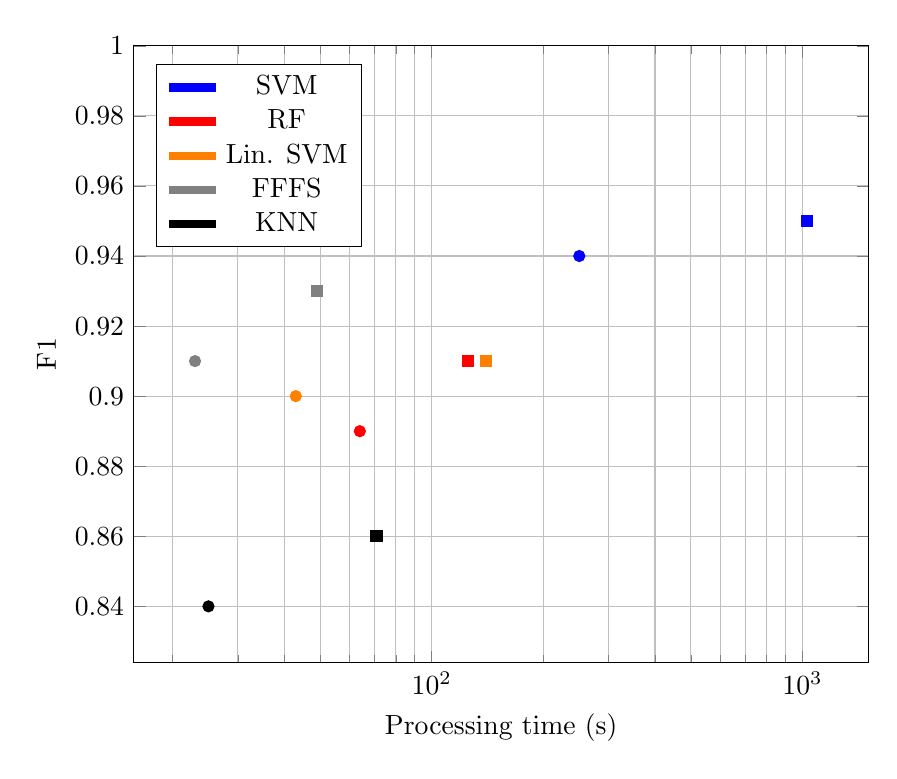
\begin{tikzpicture}
  \begin{semilogxaxis}[width=0.9\textwidth,xlabel=Processing time (s),ylabel=F1,grid=both,xmin=0,ymax=1,legend pos = north west]
  \addplot[mark size=2pt,legend image post style={sharp plot, line width=3pt, mark=none},only marks,blue,mark=*] coordinates {(250,0.94)};
  \addplot[mark size=2pt,legend image post style={sharp plot, line width=3pt, mark=none},only marks,red,mark=*] coordinates {(64,0.89)};
  \addplot[mark size=2pt,legend image post style={sharp plot, line width=3pt, mark=none},only marks,orange,mark=*] coordinates {(43,0.90)};
  \addplot[mark size=2pt,legend image post style={sharp plot, line width=3pt, mark=none},only marks,gray,mark=*] coordinates {(23,0.91)};
  \addplot[mark size=2pt,legend image post style={sharp plot, line width=3pt, mark=none},only marks,black,mark=*] coordinates {(25,0.84)};
  \legend{SVM,RF,Lin. SVM,FFFS,KNN};
  \addplot[mark size=2pt,legend image post style={sharp plot, line width=3pt, mark=none},only marks,blue,mark=square*] coordinates {(1030,0.95)};
  \addplot[mark size=2pt,legend image post style={sharp plot, line width=3pt, mark=none},only marks,red,mark=square*] coordinates {(125,0.91)};
  \addplot[mark size=2pt,legend image post style={sharp plot, line width=3pt, mark=none},only marks,orange,mark=square*] coordinates {(140,0.91)};
  \addplot[mark size=2pt,legend image post style={sharp plot, line width=3pt, mark=none},only marks,gray,mark=square*] coordinates {(49,0.93)};
  \addplot[mark size=2pt,legend image post style={sharp plot, line width=3pt, mark=none},only marks,black,mark=square*] coordinates {(71,0.86)};
  \end{semilogxaxis}
  \end{tikzpicture}
\end{center}
\end{column}
\end{columns}
\end{frame}
\begin{frame}[label={sec:org7873d16}]{Classification Map}
\begin{columns}
\begin{column}{0.5\columnwidth}
\begin{center}
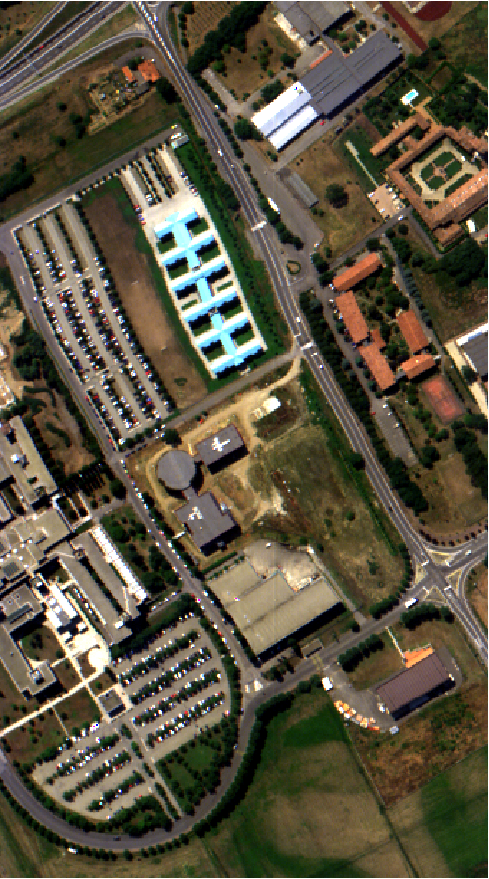
\includegraphics[width=0.55\textwidth]{./figures/university_color.png}
\end{center}
\end{column}
\begin{column}{0.5\columnwidth}
\begin{center}
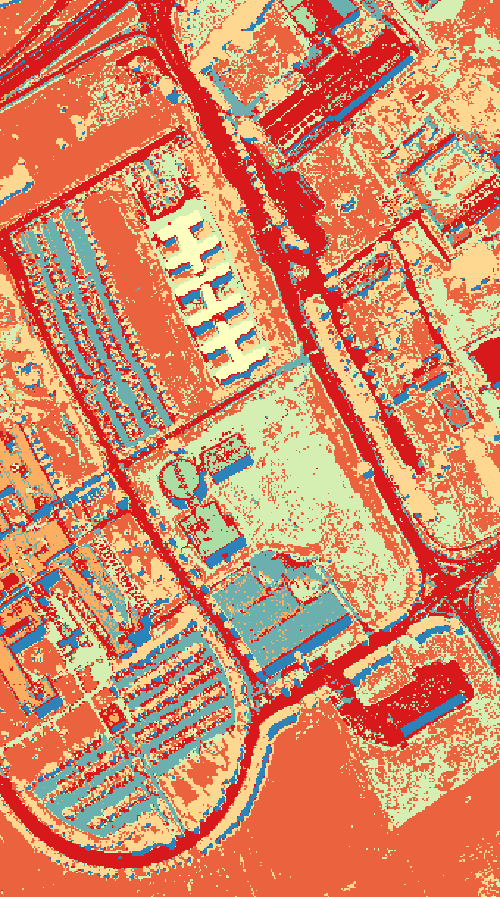
\includegraphics[width=0.55\textwidth]{./figures/university_tm_svm.png}
\end{center}
\end{column}
\end{columns}
\end{frame}

\subsection{Comparison spectral feature extraction}
\label{sec:orgf1f1899}
\begin{frame}[fragile,label={sec:orgae99823}]{PCA, LDA and KPCA}
 \begin{minted}[fontsize=\footnotesize,obeytabs=true,tabsize=4,bgcolor=bg]{python}
DATA = ['../Data/university.tif','../Data/pca_university.tif','../Data/lda_university.tif',
        '../Data/kpca_university.tif']
GT = '../Data/university_gt.tif'

F1_knn,F1_gmm = [],[]
for data in DATA:
    print data
    # Load data set
    X,y=rt.get_samples_from_roi(data,GT)
    sc = StandardScaler()
    X = sc.fit_transform(X)
\end{minted}
\begin{center}
  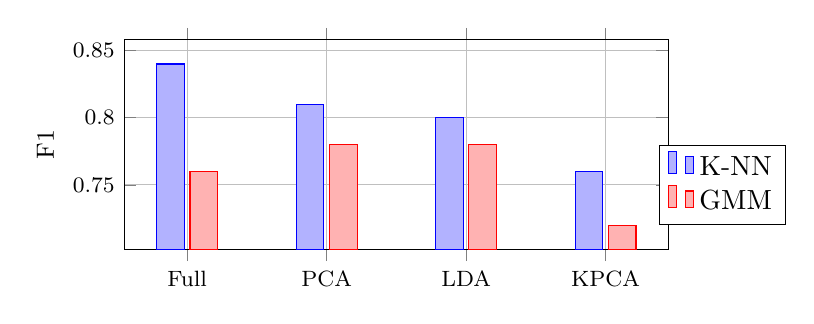
\begin{tikzpicture}
    \begin{axis}[ybar,small,enlargelimits=0.15, legend style={at={(1.1,0.5)},anchor=north},
      ylabel={F1},
      symbolic x coords={Full,PCA,LDA,KPCA},
      xtick=data, width=0.7\textwidth,height=0.35\textwidth,grid]
      \addplot coordinates {(Full,0.84) (PCA,0.81) (LDA,0.80) (KPCA,0.76)};
      \addplot coordinates {(Full,0.76) (PCA,0.78) (LDA,0.78) (KPCA,0.72)};
      \legend{K-NN,GMM}
    \end{axis}
  \end{tikzpicture}
\end{center}
\end{frame}
\section{Spatial-spectral Classification}
\label{sec:org71c2fd9}
\subsection{Introduction}
\label{sec:org068b131}
\begin{frame}[label={sec:org5a151af}]{Overview of spatial-spectral methods}
\begin{columns}
\begin{column}{0.5\columnwidth}
\begin{block}{Spatial inter-pixel dependency}
\begin{itemize}
\item Spatial feature extraction
\begin{itemize}
\item Texture
\item Mathematical morphology
\item Convolution
\end{itemize}
\item Image Segmentation
\begin{itemize}
\item kmeans
\item MeanShift
\end{itemize}
\item Markov Random Field
\end{itemize}

\vspace{0.45cm}
\end{block}
\end{column}

\begin{column}{0.5\columnwidth}
\begin{block}<only@2>{Joint use of spectral and spatial information}
\begin{itemize}
\item Data fusion
\begin{itemize}
\item Input: Feature stacking,
\item Output: fusion of classifier outputs.
\end{itemize}
\item Post classification regularization
\begin{itemize}
\item Majority vote,
\item Region growing from markers.
\end{itemize}
\item Spatial-spectral classifiers:
\begin{itemize}
\item Composite kernel
\item MRF
\end{itemize}
\end{itemize}
\end{block}
\end{column}
\end{columns}
\end{frame}
\begin{frame}[label={sec:org326dc6c}]{Question to solve}
\begin{enumerate}
\item What kind of information is needed ?
\item How to extract it from the data ?
\item How to combine it with the spectral information ?
\end{enumerate}
\end{frame}
\subsection{Spatial filter}
\label{sec:org048cde6}
\begin{frame}[fragile,label={sec:org0b9fac8}]{Texture information}
 \begin{itemize}
\item Template filters
\begin{itemize}
\item Mean, variance, median, entropy, range, \ldots{}
\end{itemize}
\item Gabor features
\item Wavelet features \cite{1026708}
\item Co-occurrence  \cite{4309314}
\end{itemize}

\begin{minted}[fontsize=\footnotesize,obeytabs=true,tabsize=4,bgcolor=bg]{bash}
otbcli_HaralickTextureExtraction -in ../Data/pca_university.tif -channel 1 \
				 -out ../Data/university_haralick.tif -parameters.min 789 parameters.max 64897
\end{minted}

\begin{columns}
\begin{column}{0.3\columnwidth}
\begin{block}{Color Image}
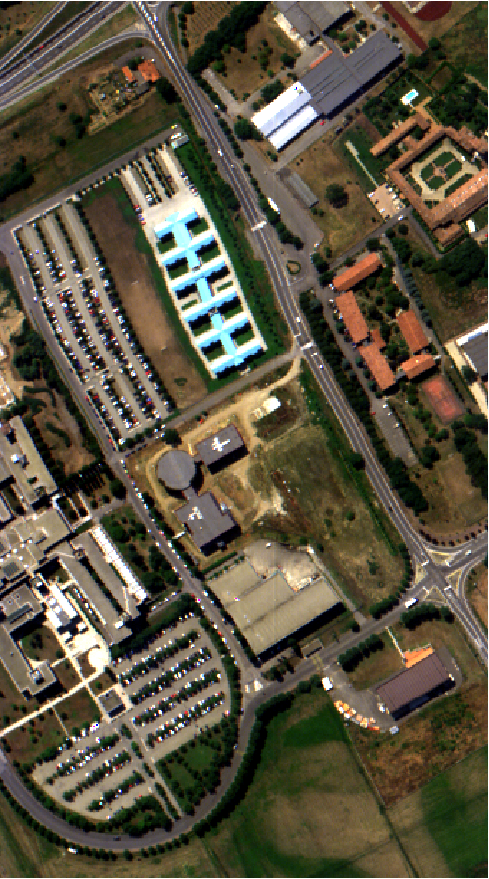
\includegraphics[trim=2.944cm 8.832cm 2.944cm 10.304cm, clip=true,width=0.9\textwidth]{./figures/university_color.png}
\end{block}
\end{column}
\begin{column}{0.3\columnwidth}
\begin{block}{Energy for PC1}
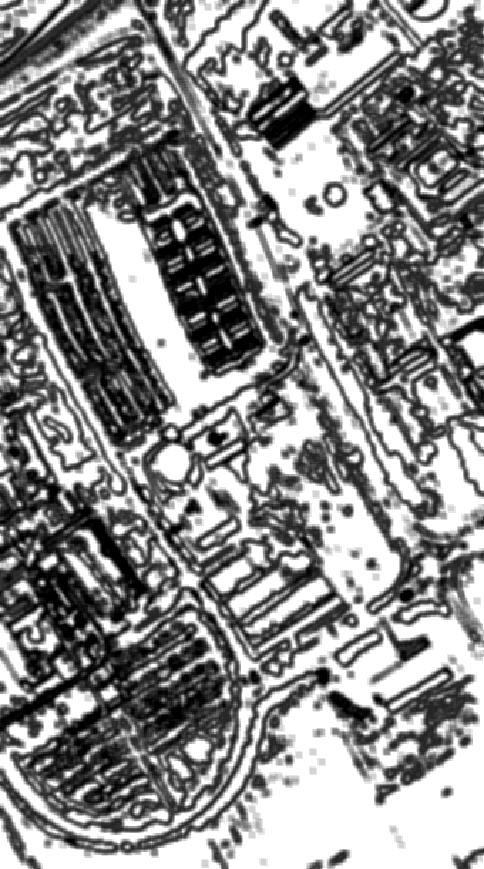
\includegraphics[trim=2.944cm 8.832cm 2.944cm 10.304cm, clip=true,width=0.9\textwidth]{./figures/university_H1.png}
\end{block}
\end{column}
\begin{column}{0.3\columnwidth}
\begin{block}{Correlation for PC1}
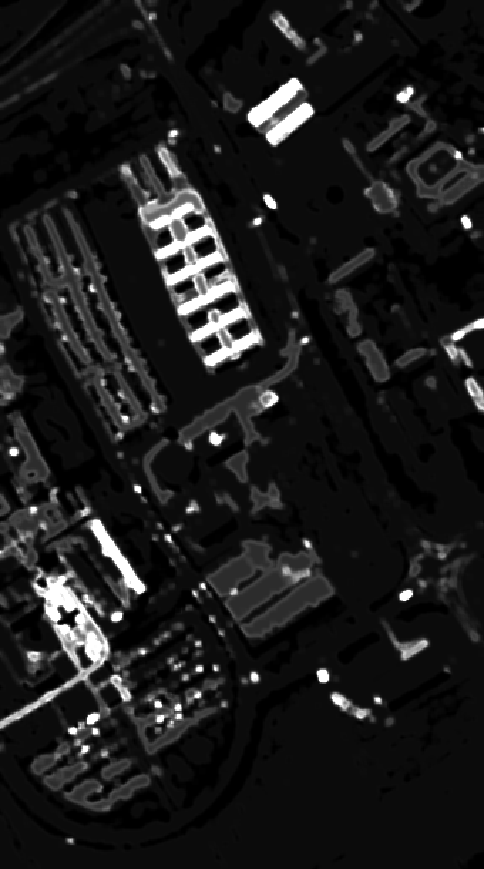
\includegraphics[trim=2.944cm 8.832cm 2.944cm 10.304cm, clip=true,width=0.9\textwidth]{./figures/university_H8.png}
\end{block}
\end{column}
\end{columns}
\end{frame}
\begin{frame}[label={sec:orge704bbf}]{Morphological neighborhood}
\begin{center}
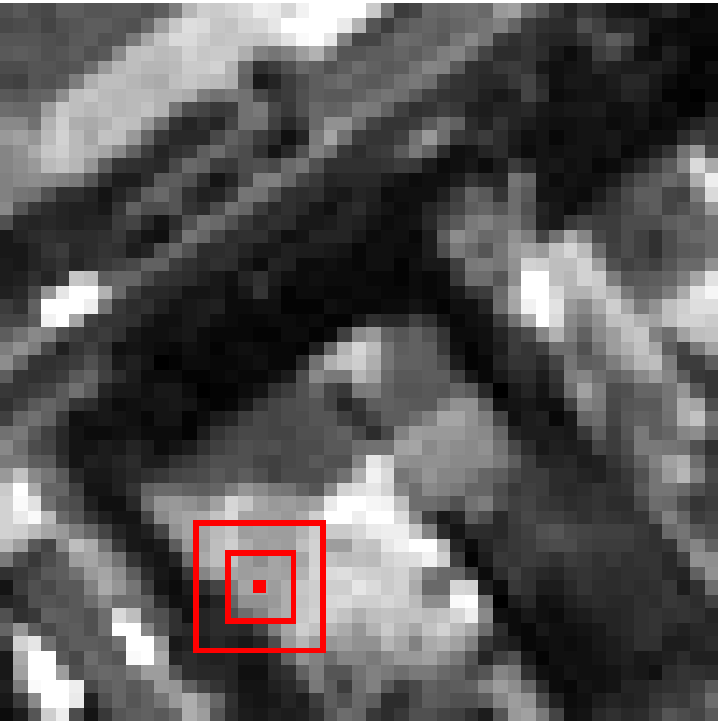
\includegraphics[trim = 0mm 0mm 0mm 40mm,clip,width=0.25\textwidth]{./figures/neighbors_1.pdf}
\end{center}

\begin{definition}[Morphological neighborhood]
The Morphological Neighborhood  of a pixel \(\mathbf{x}\) is  the set of
pixels that belongs to the same spatial structure than \(\mathbf{x}\).
\end{definition}

\begin{example}[Comparison with some neighborhood systems]
\centerline{\begin{tabular}{cccc}
    \pgfimage[width=0.30\textwidth]{figures/mrf} & \pgfimage[width=0.15\textwidth]{figures/composite} & \pgfimage[width=0.15\textwidth]{figures/texture}& \pgfimage[width=0.15\textwidth]{figures/morpho}\\ 
MRF & 8-connectivity & 4-connectivity& MN
\end{tabular}
}
\end{example}
\end{frame}

\begin{frame}[label={sec:org37d99c3}]{Morphological profile}
\begin{definition}[Morphological profile]
The Morphological  Profile of  size \(n\) is  a \((2n+1)\)-dimensional
vector such as:\vspace{-0.25cm}
$$\text{MP}(\mathbf{x})=\Big[\text{CP}_n(\mathbf{x}),f(\mathbf{x}),\text{OP}_n(\mathbf{x})\Big].$$
\end{definition}
\begin{center}
\begin{tikzpicture}
  \draw (0,0) node  {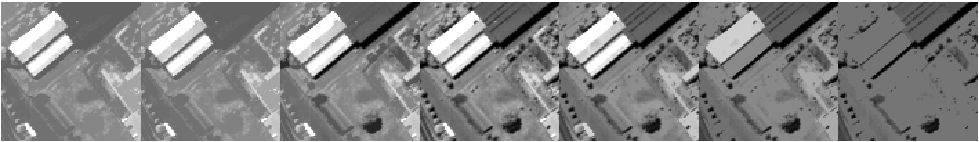
\includegraphics[width=0.9\linewidth]{figures/mp_0.pdf}};
  \draw (0,-1.25) node  {$\mathbf{x}$};
  \draw[->,thick] (0.125,-1.25) -- (0.45\linewidth,-1.25); 
  \draw[->,thick] (-0.125,-1.25) -- (-0.45\linewidth,-1.25);
  \draw[] (0.4\linewidth,-1.5) node {OP($\mathbf{x}$)}; 
  \draw[] (-0.4\linewidth,-1.5) node {CP($\mathbf{x}$)}; 
\end{tikzpicture}
\end{center}

For a given pixel \(\mathbf{x}\), information include in the MP(\(\mathbf{x}\)) are:
\begin{itemize}
\item <2>  \uline{Contrast}: Is  the structure to which the pixel  belongs to  darker or  lighter than his surrounding neighbors?
\item <2> \uline{Size}:  Is the structure to which the  pixel belongs to  small or big compared to \(G\)?
\end{itemize}
\end{frame}
\begin{frame}[label={sec:orgcf3c859}]{Derivative of the MP}
\begin{definition}[Derivative of the morphological profile]
The  Derivative  of  the  Morphological  Profile  of  size  \(n\)  is  a \((2n)\)-dimensional vector such as:\vspace{-0.25cm}

$$\text{DMP}(\mathbf{x})=\Big[|\phi_n(\mathbf{x})-\phi_{n-1}(\mathbf{x})|,\ldots,|\gamma_{n-1}(\mathbf{x})-\gamma_n(\mathbf{x})|\Big].$$
\end{definition}
\begin{center}
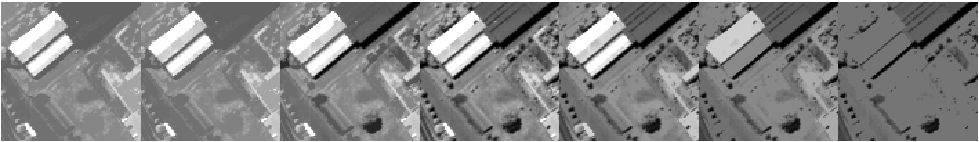
\includegraphics[width=0.9\textwidth,height=0.15\textwidth]{./figures/mp_0.pdf}
\end{center}

\begin{center}
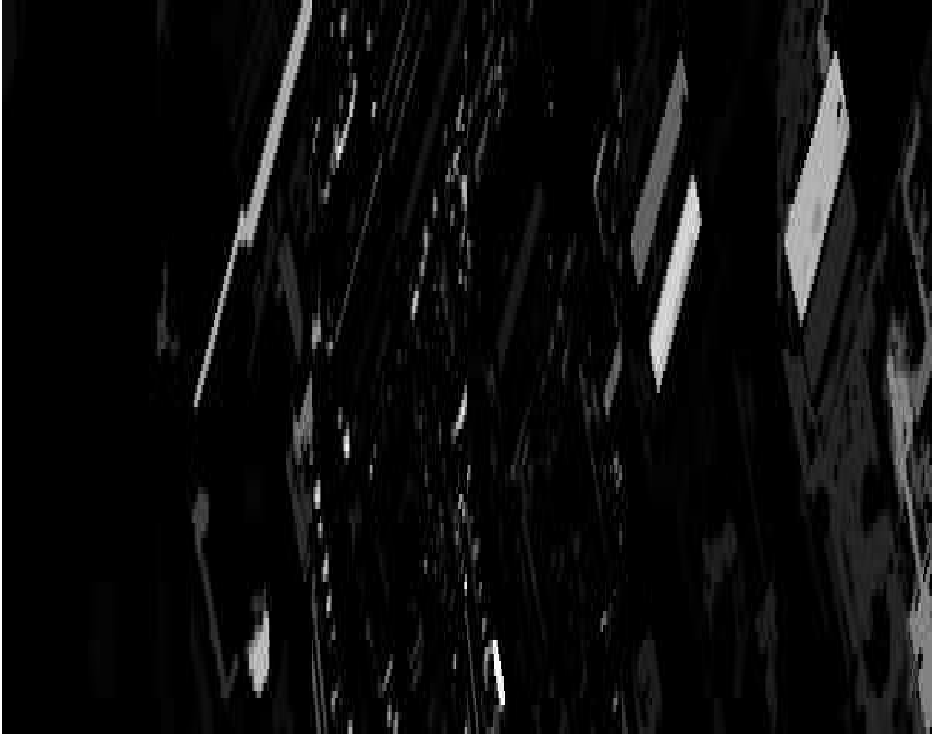
\includegraphics[width=0.75\textwidth,height=0.15\textwidth]{./figures/DMP_im.pdf}
\end{center}
\end{frame}
\begin{frame}[label={sec:org3aec75c}]{Limits of the (D)MP}
\begin{itemize}
\item Geodesics filters only act on extrema structures
\item <4> Self-complementary area filter
\end{itemize}


\only<1>{\centerline{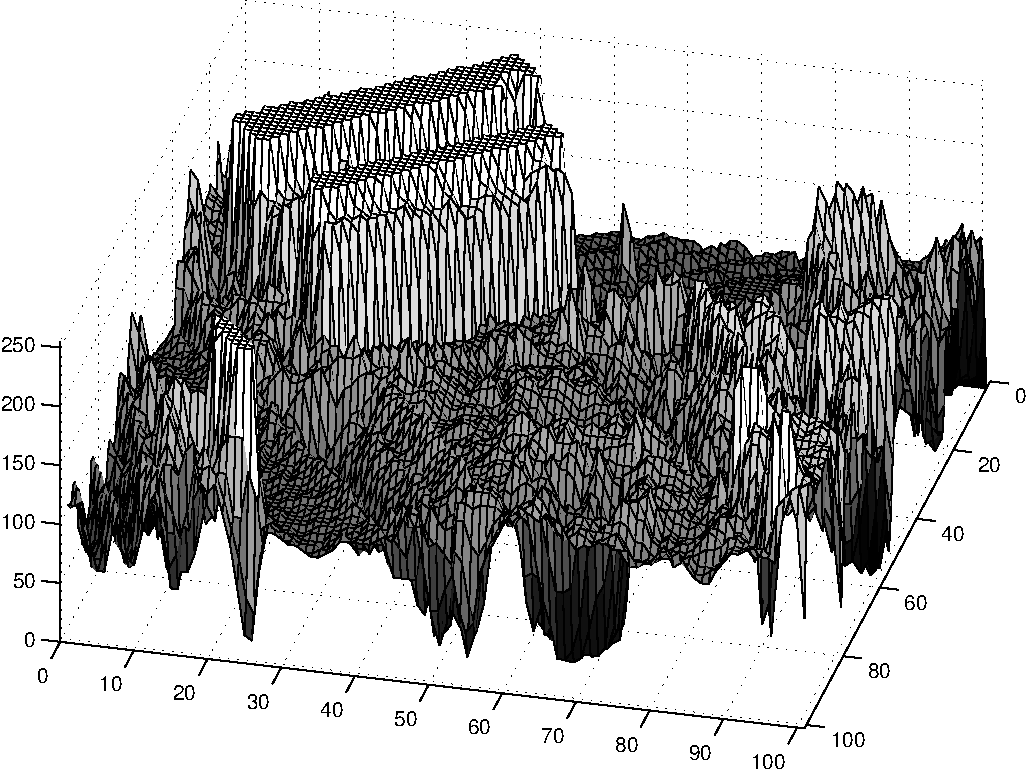
\includegraphics[width=0.60\textwidth]{figures/orig_g}}}
\only<2>{\centerline{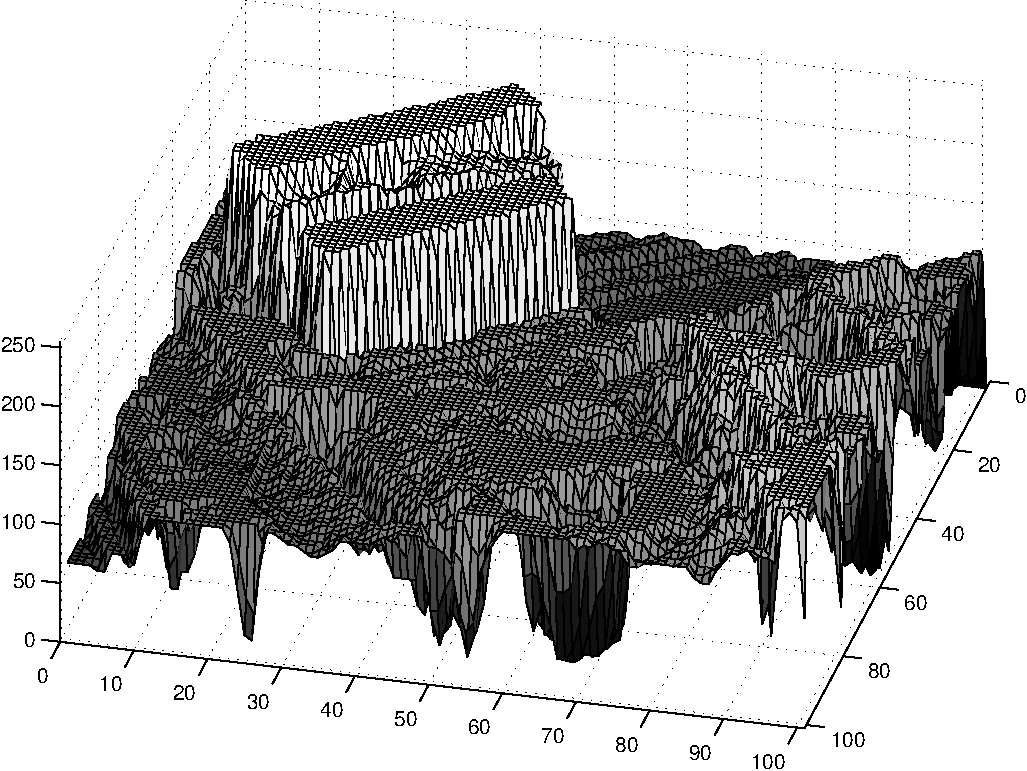
\includegraphics[width=0.60\textwidth]{figures/open_g}}}
\only<3>{\centerline{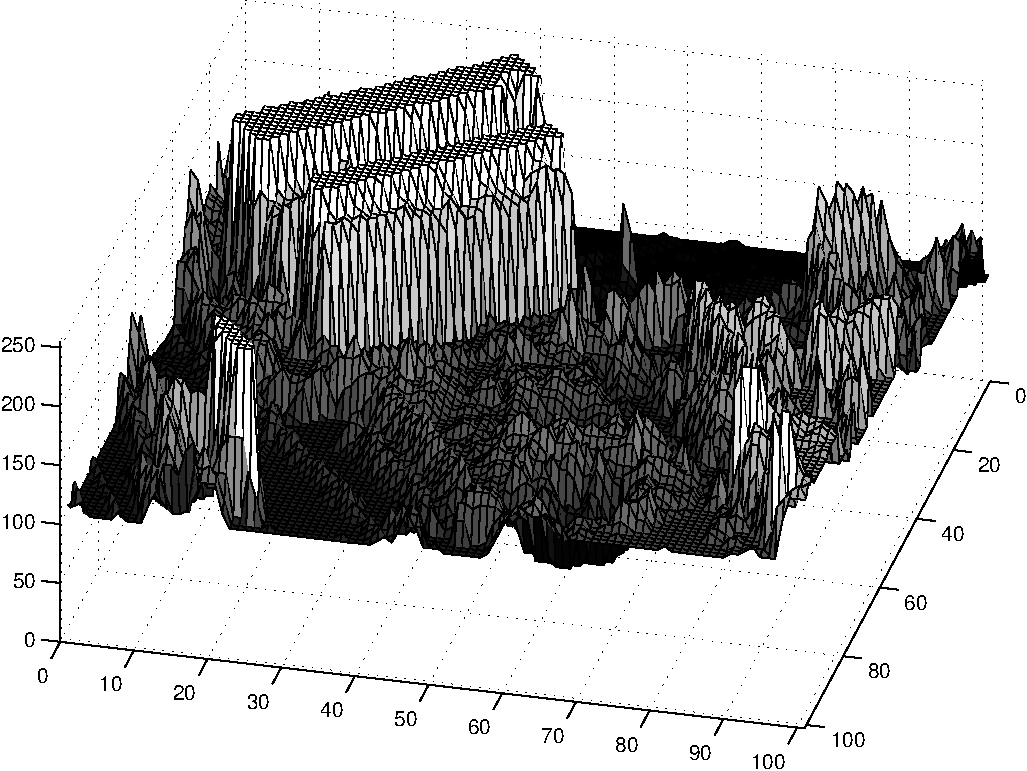
\includegraphics[width=0.60\textwidth]{figures/close_g}}}
\only<4>{\centerline{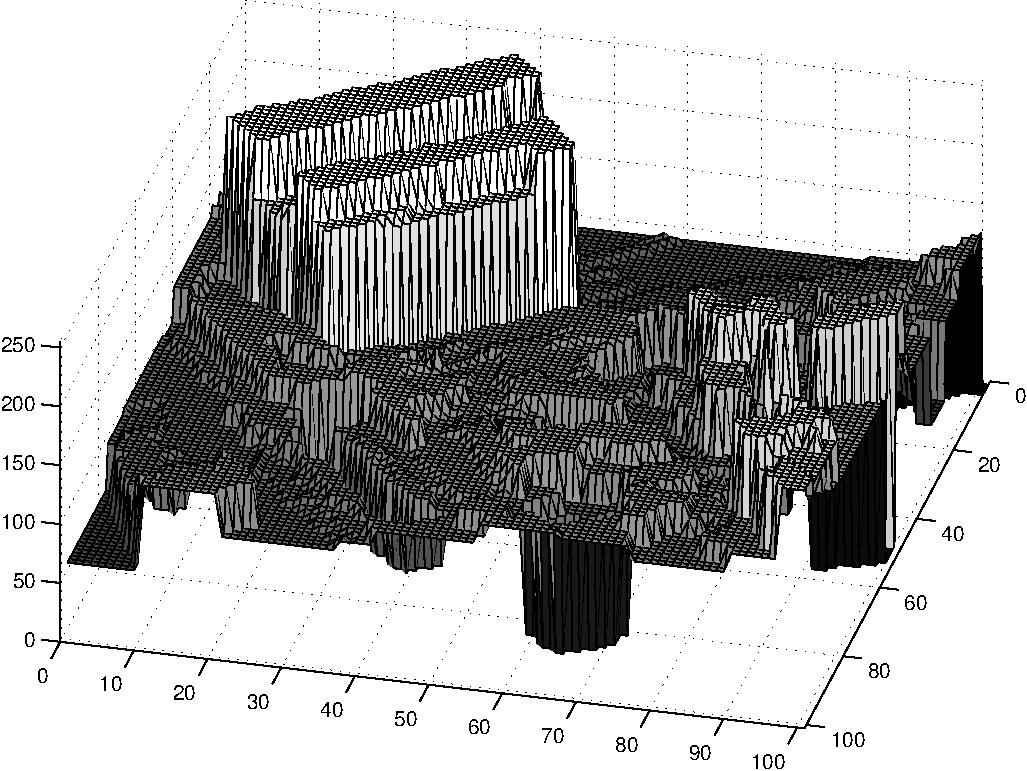
\includegraphics[width=0.60\textwidth]{figures/area_g}}}
\end{frame}
\begin{frame}[label={sec:org5e51259}]{Self-complementary area filter}
\begin{itemize}
\item Self-complementarity: \(\Psi = \mathbf{C}\Psi\Rightarrow\) each structure is processed equally.
\item Area filter: Removes small structures (area = number of pixels).
\item Algorithm:
\begin{enumerate}
\item Label all the flat zones that satisfy the area criterion \(\lambda\),
\item Grow  the labelled flat  zones until a partition  of the image is reached.
\end{enumerate}
\end{itemize}

\centerline{
\begin{tabular}{c@{~}c@{~}c@{~}c}
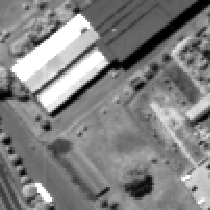
\includegraphics[width=0.23\textwidth,height=0.23\textwidth]{figures/orig.pdf} & 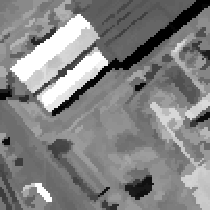
\includegraphics[width=0.23\textwidth,height=0.23\textwidth]{figures/image_filtree_10}& 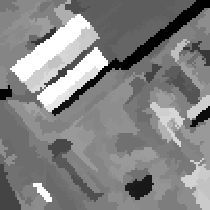
\includegraphics[width=0.23\textwidth,height=0.23\textwidth]{figures/image_filtree_30}& 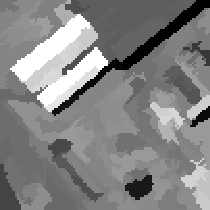
\includegraphics[width=0.23\textwidth,height=0.23\textwidth]{figures/image_filtree_40}\\
Original & $\lambda =10$ & $\lambda =30$ & $\lambda =40$
\end{tabular}}
\end{frame}
\begin{frame}[label={sec:org211929d}]{MN based on area filtering}
\begin{itemize}
\item Extract the inter-pixel dependency \(\Upsilon\):

\centerline{
    \begin{tabular}{c@{~}c@{~}c}
      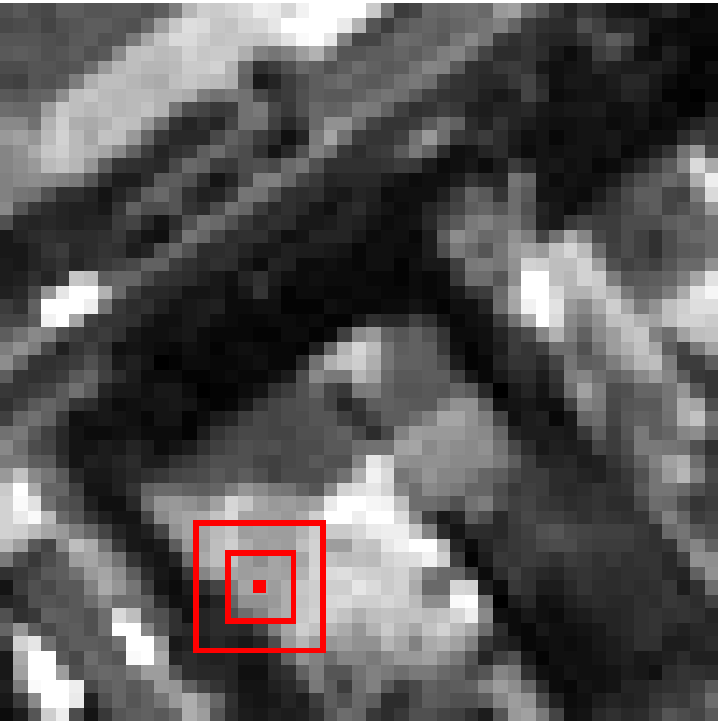
\includegraphics[width=0.25\textwidth]{figures/neighbors_1}&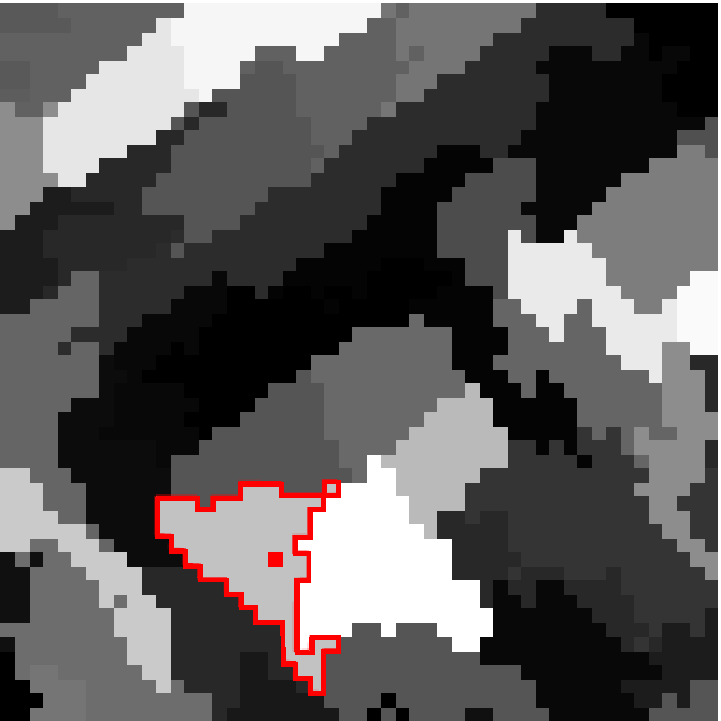
\includegraphics[width=0.25\textwidth]{figures/neighbors_2}&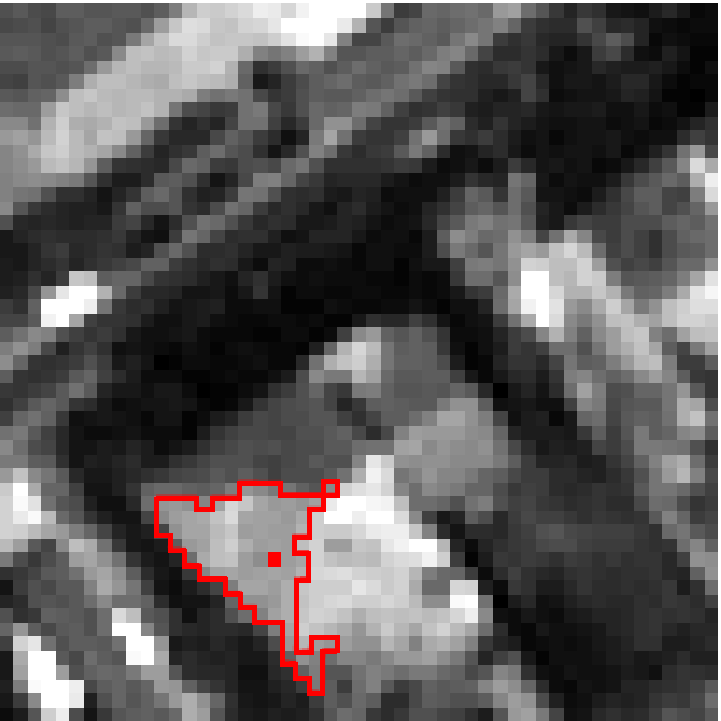
\includegraphics[width=0.25\textwidth]{figures/neighbors_3}\\
      \color{red}$\mathbf{x}$& $\lambda=30$ & \color{red}$\Omega_\mathbf{x}$
    \end{tabular}
  }
\item \(\Upsilon_\mathbf{x}=\text{median}(\Omega_\mathbf{x})\):
\begin{itemize}
\item Structure: What are the pixels related to \(\mathbf{x}\)?
\item Contrast: Local gray-level distribution
\end{itemize}
\end{itemize}
\end{frame}
\begin{frame}[label={sec:org1fe5a3e}]{Extended Morphological Profile}
\begin{definition}[Extended Morphological Profile]
The EMP of  size \(n\times p\) is a  \((2n+1)p\)-dimensional vector made
of   the  MP   build  with   the  \(p\)   first  principal   components:
$$\text{EMP}(\mathbf{x})=\Big[\text{MP}_1(\mathbf{x}),\ldots,\text{MP}_p(\mathbf{x})\Big].$$
\end{definition}
\centerline{\resizebox{0.95\textwidth}{!}{\input{figures/emp.pdf_t}}}

\begin{itemize}
\item Fusion of morphological and spectral features
\item PCA, FDA, Kernel-PCA \ldots{}
\item \emph{Same methods for self-complementary area filter}
\end{itemize}
\end{frame}

\begin{frame}[fragile,label={sec:org3ba0690}]{Application case: Extended Morphological Profile}
 \begin{minted}[fontsize=\footnotesize,obeytabs=true,tabsize=4,bgcolor=bg]{python}
    # Start the computation
    for i in xrange(no):
        # Structuring elements
        se = disk(radius+i*2)

        # Compute opening per reconstruction
        temp = erosion(im,se)
        out[:,:,no+1+i] = reconstruction(temp,im,method='dilation')

        # Compute closing per reconstruction
        temp = dilation(im,se)
        out[:,:,no-1-i] = reconstruction(temp,im,method='erosion')

    return out
\end{minted}
\begin{minted}[fontsize=\footnotesize,obeytabs=true,tabsize=4,bgcolor=bg]{python}
if __name__ == '__main__':
    # Load image
    im,GeoT,Proj = rt.open_data('../Data/pca_university.tif')

    # Apply the Morphological profile on each PC
    EMP = []
    for i in xrange(3):
        EMP.append(morphological_profile(im[:,:,i]))
    EMP = sp.concatenate(EMP,axis=2)
    rt.write_data("../Data/emp_pca_university.tif",EMP,GeoT,Proj)
\end{minted}
\end{frame}
\begin{frame}[label={sec:org44e820e}]{Questions 1/2}
\begin{columns}
\begin{column}{0.5\columnwidth}
\begin{center}
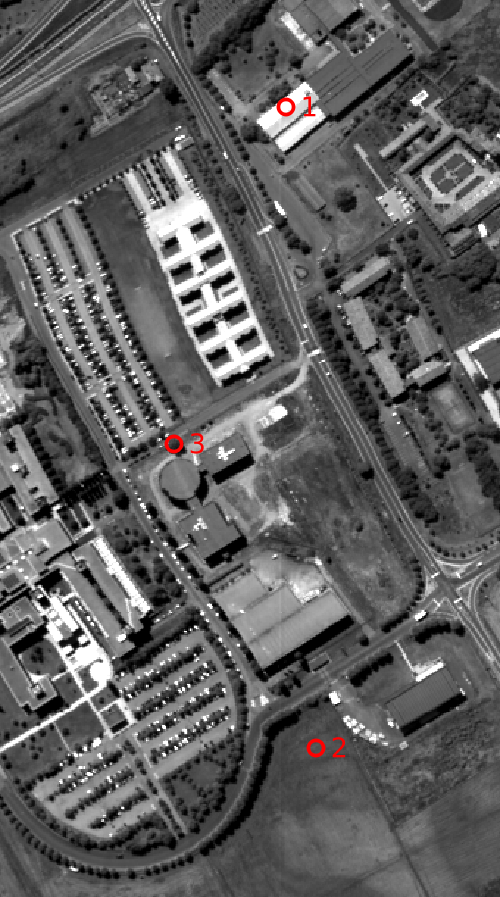
\includegraphics[width=0.6\textwidth]{./figures/emp_question.png}
\end{center}
\end{column}

\begin{column}{0.5\columnwidth}
\begin{center}
  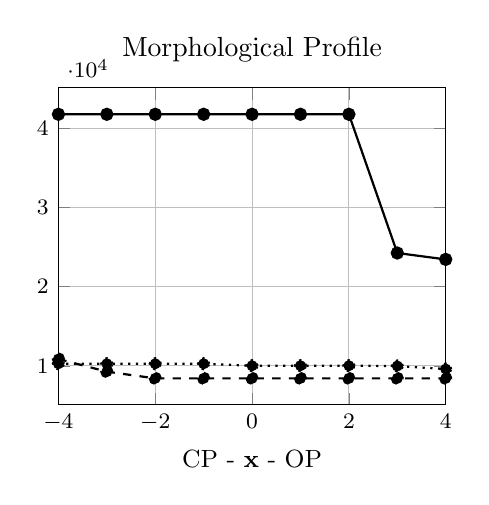
\begin{tikzpicture}
    \begin{axis}[grid,xmin=-4,xmax=4,small,cycle list name=linestyles,title=Morphological Profile,xlabel=CP - $\mathbf{x}$ - OP]
      \addplot+[mark=*,thick] coordinates {(-4,41772) (-3,41772) (-2,41772) (-1,41772) (0,41772) (1,41772) (2,41772) (3,24257) (4,23449)} ;      
      \addplot+[mark=*,thick] coordinates {(-4,10876) (-3,9277) (-2,8430) (-1,8430) (0,8430) (1,8430) (2,8430) (3,8430) (4,8430)} ;
      \addplot+[mark=*,thick] coordinates {(-4,10276) (-3,10276) (-2,10276) (-1,10276) (0,10026) (1,10026) (2,10026) (3,9991) (4,9608)} ;  
    \end{axis}
  \end{tikzpicture}
\end{center}
\end{column}
\end{columns}
\end{frame}

\begin{frame}[label={sec:orge9d3f3f}]{Questions 2/2}
Where is the \emph{closing} and the \emph{opening} ?
\begin{columns}
\begin{column}{0.3\columnwidth}
\begin{center}
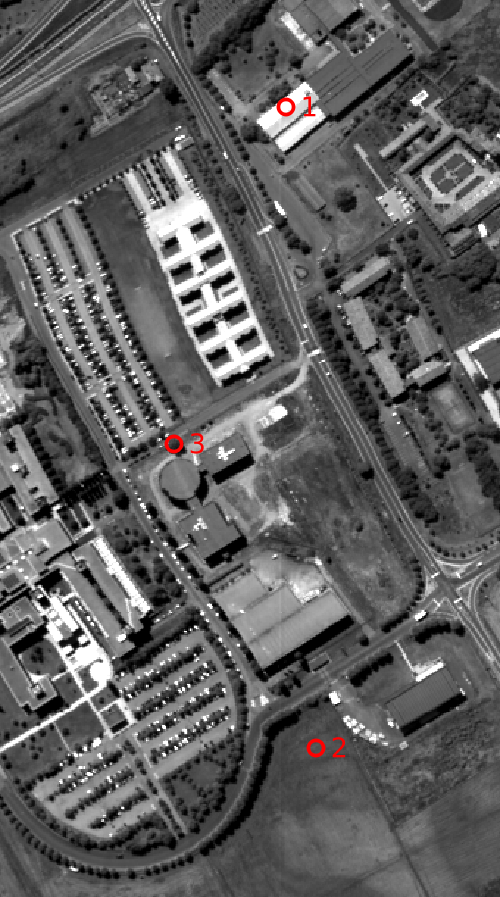
\includegraphics[width=0.8\textwidth]{./figures/emp_question.png}
\end{center}
\end{column}

\begin{column}{0.3\columnwidth}
\begin{center}
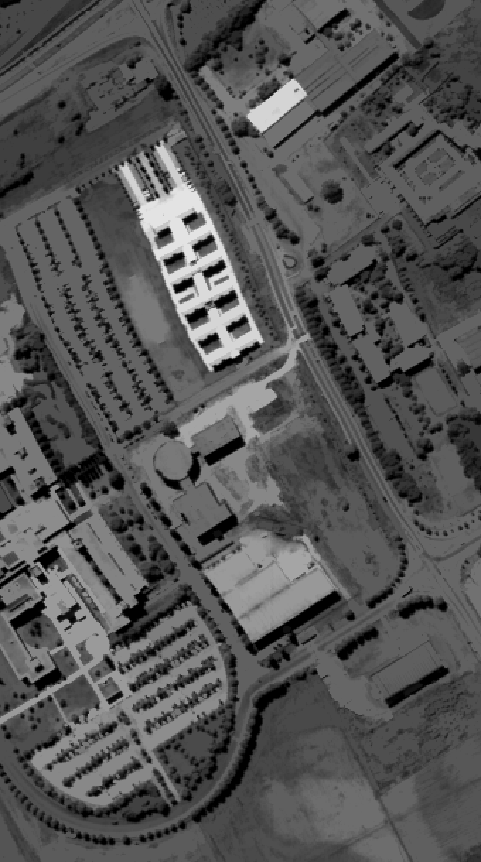
\includegraphics[width=0.8\textwidth]{./figures/university_opening.png}
\end{center}
\end{column}

\begin{column}{0.3\columnwidth}
\begin{center}
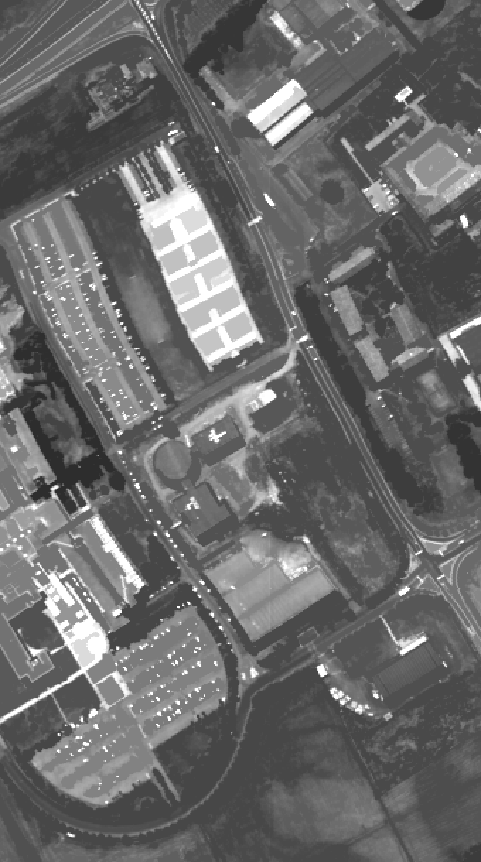
\includegraphics[width=0.8\textwidth]{./figures/university_closing.png}
\end{center}
\end{column}
\end{columns}
\end{frame}

\subsection{Data fusion}
\label{sec:org17c9116}
\begin{frame}[label={sec:org5292eba}]{Feature fusion 1/2}
\begin{center}
  \tikzstyle{data} = [draw, ellipse,fill=red!20, node distance=3cm, minimum height=2em]
  \tikzstyle{block} = [rectangle, draw, fill=blue!20,text width=5em, text centered, rounded corners, minimum height=4em]
  \tikzstyle{line} = [draw, -latex']
  \begin{tikzpicture}
    \draw (0,2) node[data] (F1) {Feature 1};
    \draw (0,1) node[data] (F2) {Feature 2};
    \draw (0,0) node[] {$\vdots$};
    \draw (0,-1) node[data] (Fk) {Feature k};
    \draw (0,-2) node[data] (FK) {Feature K};
    \draw (4,0) node[block] (stack) {Stacking};
    \draw (8,0) node[block] (class) {Classifier};
    \path [line] (F1) -- (stack);
    \path [line] (F2) -- (stack);
    \path [line] (Fk) -- (stack);
    \path [line] (FK) -- (stack);
    \path [line] (stack) -- (class);
  \end{tikzpicture}
\end{center}
\end{frame}
\begin{frame}[label={sec:org4674f3e}]{Feature fusion 2/2}
\begin{columns}
\begin{column}{0.5\columnwidth}
\begin{itemize}
\item Extract several spatial descriptors
\begin{itemize}
\item EMP,
\item Texture,
\item Histogram of oriented gradients (HOG),
\item \ldots{}
\end{itemize}
\item \emph{Optional}: apply feature extraction 
\begin{itemize}
\item Spectral features,
\item Spatial features,
\item Both
\end{itemize}
\item Stack all the features into a "big vector"
\end{itemize}
\end{column}

\begin{column}{0.5\columnwidth}
\begin{itemize}
\item In \cite{fauvel2008spectral}:
\begin{itemize}
\item Extrat EMP
\item Apply PCA/LDA to the spectral and spatial features
\item Stack the first PCs of spectral/spatial feautres
\item Classification with SVM
\end{itemize}
\end{itemize}
\begin{center}
\begin{tabular}{lrr}
\toprule
Method & \# Features & OA\\
\midrule
Spectral & 103 & 79.5\\
EMP & 27 & 79.1\\
S+EMP & 130 & 83.5\\
S-DBFE+EMP-DBFE & 27+10 & 88.0\\
\bottomrule
\end{tabular}
\end{center}
\end{column}
\end{columns}
\end{frame}
\begin{frame}[label={sec:org8ad355a}]{Classifier fusion 1/2}
\begin{center}
  \tikzstyle{data} = [draw, ellipse,fill=red!20, node distance=3cm, minimum height=2em]
  \tikzstyle{block} = [rectangle, draw, fill=blue!20,text width=5em, text centered, rounded corners, minimum height=2em]
  \tikzstyle{line} = [draw, -latex']
  \begin{tikzpicture}
    \draw (0,2) node[data] (F1) {Feature 1};
    \draw (0,1) node[data] (F2) {Feature 2};
    \draw (0,0) node[] {$\vdots$};
    \draw (0,-1) node[data] (Fk) {Feature k};
    \draw (0,-2) node[data] (FK) {Feature K};
    \draw (4,2) node[block] (class1) {Classifier 1};
    \draw (4,1) node[block] (class2) {Classifier 2};
    \draw (4,-1) node[block] (classk) {Classifier k};
    \draw (4,-2) node[block] (classK) {Classifier K};
    \draw (8,0) node[block] (fusion) {Fusion};
    \path [line] (F1) -- (class1);
    \path [line] (F2) -- (class2);
    \path [line] (Fk) -- (classk);
    \path [line] (FK) -- (classK);
    \path [line] (class1) -- (fusion);
    \path [line] (class2) -- (fusion);
    \path [line] (classk) -- (fusion);
    \path [line] (classK) -- (fusion);
  \end{tikzpicture}
\end{center}
\end{frame}
\begin{frame}[label={sec:org0b3c8ab}]{Classifier fusion 2/2}
\begin{columns}
\begin{column}{0.5\columnwidth}
\begin{itemize}
\item Fusion of classifier outputs:
\begin{itemize}
\item At the decision level
$$ C_1:\{y_1\};$$
$$C_2:\{y_2\};$$
$$\vdots$$
$$C_K:\{y_K\}$$
\item At the membership level
$$ C_1:\{m_{11},\ldots,m_{1C}\};$$
$$C_2:\{m_{21},\ldots,m_{2C}\};$$
$$\vdots$$
$$C_K:\{m_{K1},\ldots,m_{KC}\}$$
\end{itemize}
\item Decision level: Majority vote
\item Membership level: Probabilistics methods, fuzzy logic, Dempster-Shafer \ldots{}
\end{itemize}
\end{column}

\begin{column}{0.5\columnwidth}
\begin{itemize}
\item In \cite{Fauvel06acombined}: Fusion of SVM
\item Use the distance to the hyperplane
\item \emph{Absolute maximum} fusion rule
\item Two classifiers with different intputs: Spectral and EMP
\end{itemize}
\begin{center}
\begin{tabular}{lr}
\toprule
Feature & OA\\
\midrule
Spectral & 81.0\\
EMP & 85.2\\
\midrule
Output fusion & 89.6\\
\bottomrule
\end{tabular}
\end{center}
\end{column}
\end{columns}
\end{frame}

\begin{frame}[fragile,label={sec:orgd1ee8f0}]{Data fusion in action}
 \begin{itemize}
\item Simple to implement:
\end{itemize}
\begin{minted}[fontsize=\footnotesize,obeytabs=true,tabsize=4,bgcolor=bg]{python}
# Concatenate the spectral and spatial features and do scaling
IM_EMP = sp.concatenate((im[:,::2],EMP.astype(im.dtype)),axis=1)
\end{minted}
\begin{itemize}
\item Good classification accuracy: \(F1=0.99\)
\item sptial
\end{itemize}

\begin{columns}
\begin{column}{0.3\columnwidth}
\begin{block}{Color Image}
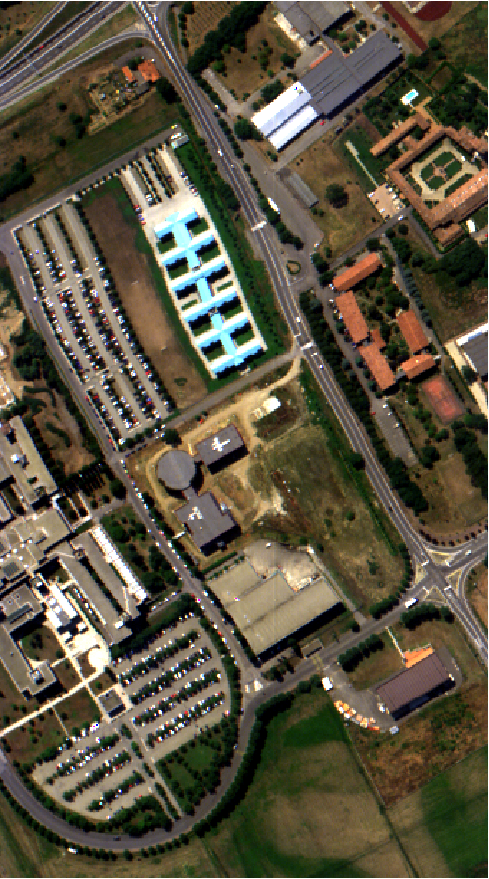
\includegraphics[trim=2.cm 1cm 2cm 14.304cm, clip=true,width=\textwidth,height=0.8\textwidth]{./figures/university_color.png}
\end{block}
\end{column}
\begin{column}{0.3\columnwidth}
\begin{block}{Spectral only}
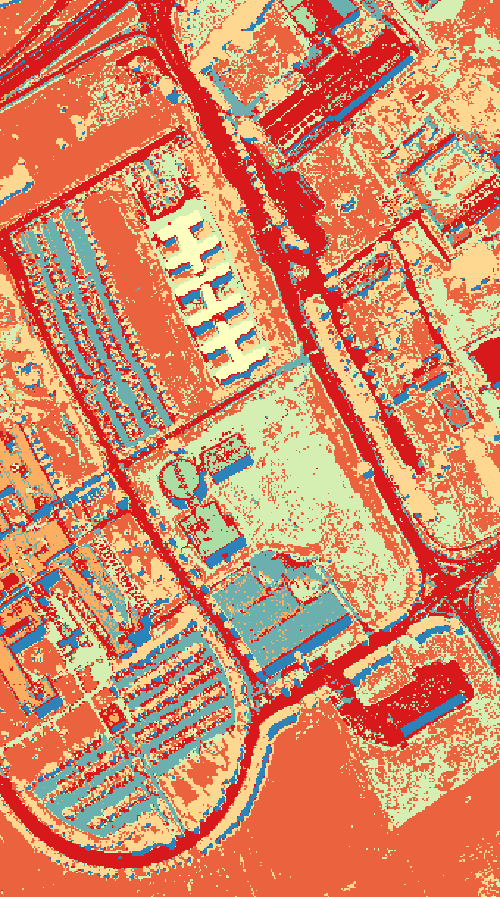
\includegraphics[trim=2.cm 1cm 2cm 14.304cm, clip=true,width=\textwidth,height=0.8\textwidth]{./figures/university_tm_svm.png}
\end{block}
\end{column}
\begin{column}{0.3\columnwidth}
\begin{block}{Spectral + EMP}
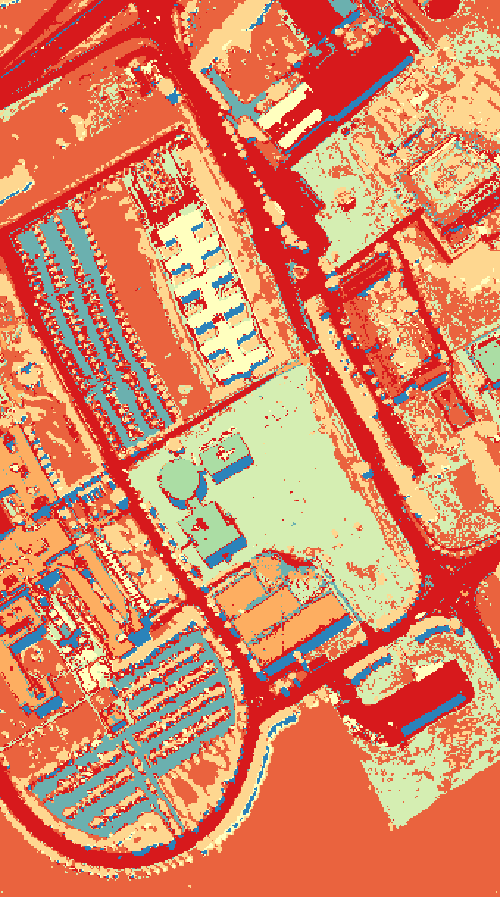
\includegraphics[trim=2.cm 1cm 2cm 14.304cm, clip=true,width=\textwidth,height=0.8\textwidth]{./figures/university_tm_fusion.png}
\end{block}
\end{column}
\end{columns}
\end{frame}
\subsection{Spatial post-regularization}
\label{sec:org785ef7c}
\begin{frame}[label={sec:orgb23ba82}]{Segmentation 1/4}
\begin{itemize}
\item Main ideas
\begin{itemize}
\item Segmentation of the image: partition the image into non-overlapping homogeneous zones
\item Spatial regularization of the thematic map
\end{itemize}
\item Issues:
\begin{itemize}
\item Segmentation of hyperspectral images is tricky !
\item Spatial regularization
\end{itemize}
\item From \cite{fauvel2013advances}:
\begin{itemize}
\item Segmentation:
\begin{itemize}
\item Image processing: Watershed, region growing, mean-shift, \ldots{}
\item Statistical: GMM, K-means \ldots{}
\end{itemize}
\item Regularization:
\begin{itemize}
\item Majority voting,
\item Region growing
\end{itemize}
\end{itemize}
\end{itemize}
\end{frame}
\begin{frame}[fragile,label={sec:org36bb8a2}]{Segmentation 2/4}
 \begin{minted}[fontsize=\footnotesize,obeytabs=true,tabsize=4,bgcolor=bg]{bash}
# Using Mean Shift
otbcli_Segmentation -in ../Data/pca_university.tif -mode raster -mode.raster.out ../Data/mean_shift_university.tif \
		    -filter.meanshift.minsize 50
\end{minted}
\begin{columns}
\begin{column}{0.4\columnwidth}
\begin{block}{Color Image}
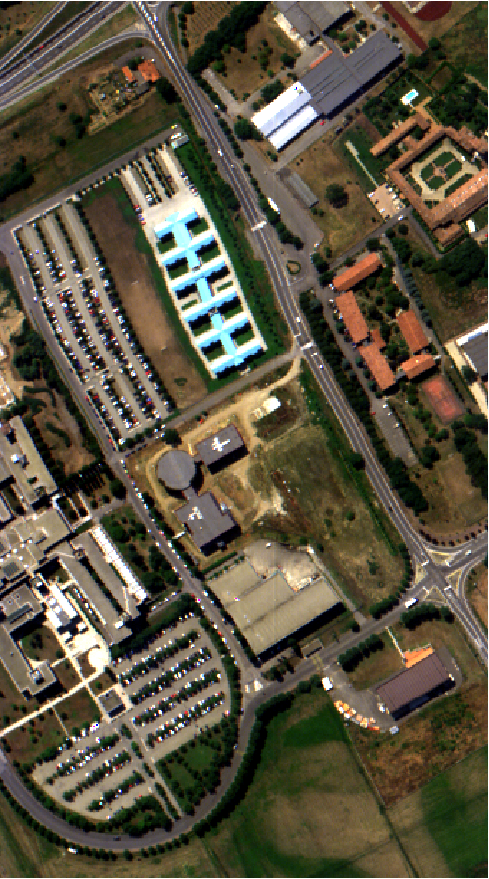
\includegraphics[trim=2.cm 1cm 2cm 14.304cm, clip=true,width=\textwidth,height=0.8\textwidth]{./figures/university_color.png}
\end{block}
\end{column}


\begin{column}{0.4\columnwidth}
\begin{block}{Segmented}
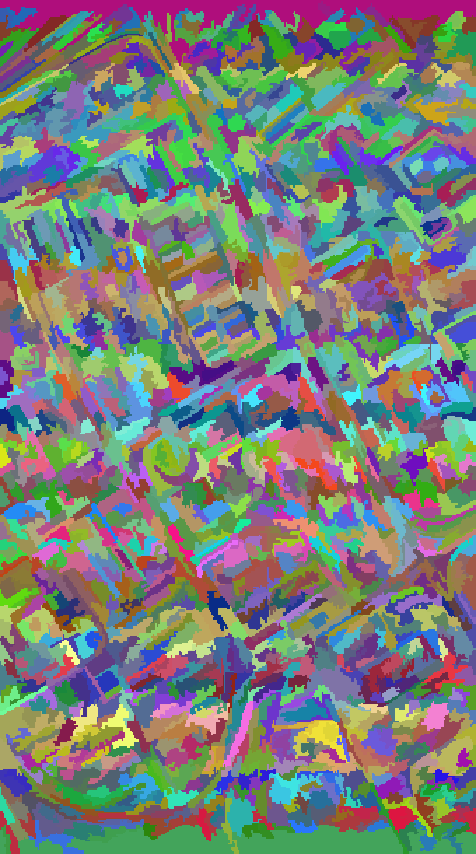
\includegraphics[trim=2.cm 1cm 2cm 14.304cm, clip=true,width=\textwidth,height=0.8\textwidth]{./figures/university_mean_shift.png}
\end{block}
\end{column}
\end{columns}
\end{frame}

\begin{frame}[fragile,label={sec:org58ca90c}]{Segmentation 3/4}
 \begin{minted}[fontsize=\footnotesize,obeytabs=true,tabsize=4,bgcolor=bg]{python}
import rasterTools as rt
import scipy as sp
from scipy.stats import mode

# Load Thematic Map
im,GeoT,Proj = rt.open_data('../Data/tm_university_svm.tif')
out = sp.empty_like(im)

# Load segmented image
segmented,GeoT,Proj = rt.open_data('../Data/mean_shift_university.tif')

# Do the majority vote
for l in sp.unique(segmented):
    t = sp.where(segmented==l)
    y = im[t]
    out[t] = mode(y, axis=None)[0][0]

# Write the new image
rt.write_data("../Data/tm_university_fusion_mv.tif",out,GeoT,Proj)
\end{minted}
\end{frame}

\begin{frame}[label={sec:org6f09e81}]{Segmentation 4/4}
\begin{columns}
\begin{column}{0.5\columnwidth}
\begin{center}
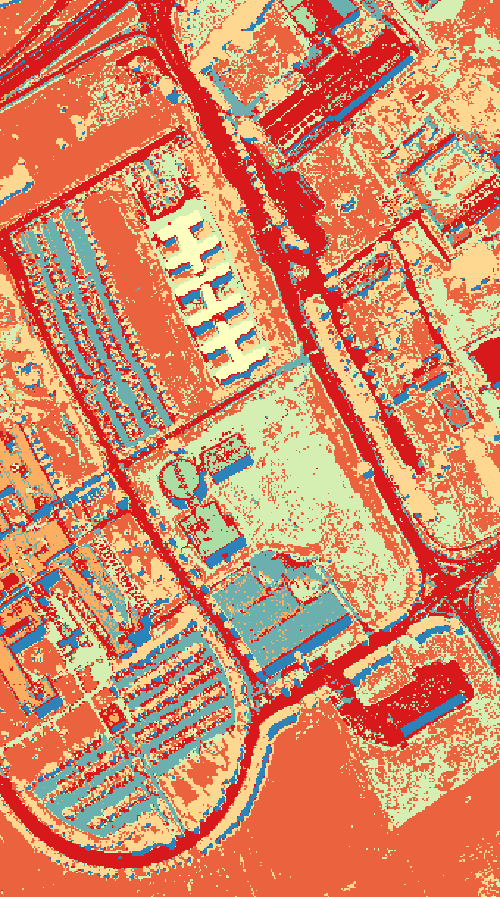
\includegraphics[width=0.6\textwidth]{./figures/university_tm_svm.png}
\end{center}
\end{column}


\begin{column}{0.5\columnwidth}
\begin{center}
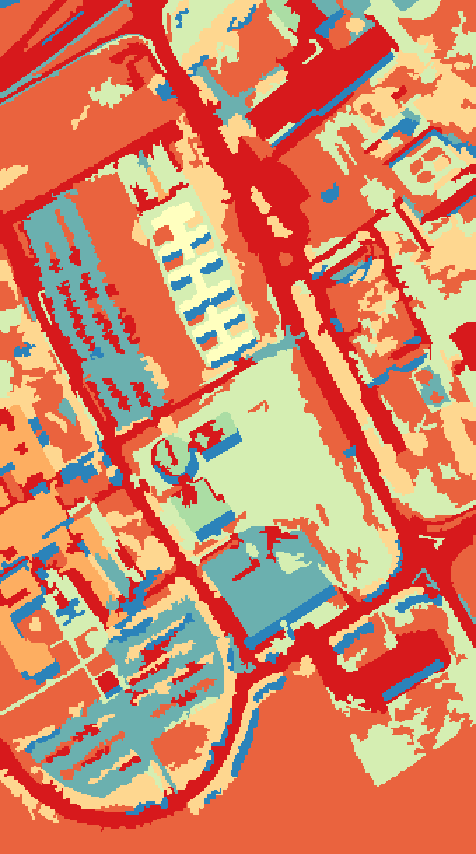
\includegraphics[width=0.6\textwidth]{./figures/university_tm_fusion_mv.png}
\end{center}
\end{column}
\end{columns}
\end{frame}

\begin{frame}[label={sec:org3665db2}]{Markov Random Field 1/2}
\begin{itemize}
\item Markovian hypothesis/condition \cite{6304904}: \(p(y_i=c|\mathbf{x}_i,\mathcal{N}_i)\)
\item \(\mathcal{N}_i\): neighborhood of pixel \(i\)
\begin{center}
      \begin{tabular}{cc}
        \tikz[baseline,scale=0.4]{\foreach \x in{-1,0,1,2,3,4}{
          \draw[] (-1,\x) -- (4,\x);
          \draw[] (\x,-1) -- (\x,4);
        }
        \draw[] (1.5,1.5) node (yi) {\small $y_{i}$};
        \filldraw[] (0.5,1.5) circle (2pt);
        \filldraw[] (2.5,1.5) circle (2pt);
        \filldraw[] (1.5,0.5) circle (2pt);
        \filldraw[] (1.5,2.5) circle (2pt);
      }&
         \tikz[baseline,scale=0.4]{\foreach \x in{-1,0,1,2,3,4}{
          \draw[] (-1,\x) -- (4,\x);
          \draw[] (\x,-1) -- (\x,4);
        }
         \draw[] (1.5,1.5) node (yi) {\small $y_{i}$};
         \filldraw[] (0.5,1.5) circle (2pt);
         \filldraw[] (0.5,0.5) circle (2pt);
         \filldraw[] (0.5,2.5) circle (2pt);
         \filldraw[] (1.5,0.5) circle (2pt);
         \filldraw[] (1.5,2.5) circle (2pt);
         \filldraw[] (2.5,0.5) circle (2pt);
         \filldraw[] (2.5,1.5) circle (2pt);
         \filldraw[] (2.5,2.5) circle (2pt);
         }\\
        First-order & Second order
      \end{tabular}
    \end{center}
\item When \(Y\) is a Markov Random Field: 
\begin{itemize}
\item \(P(Y|\mathbf{X})\propto\exp(-U(Y|\mathbf{X}))\)
\item \(U(Y|\mathbf{X})=\sum_{i=1}^nU(y_i|\mathbf{x}_i,\mathcal{N}_i)\)
\item \(U(y_i|\mathbf{x}_i,\mathcal{N}_i) = \Omega(\mathbf{x}_i,y_i) + \beta\mathcal{E}(y_i,\mathcal{N}_i)\)
\end{itemize}
\item Spectral term: \(\Omega(\mathbf{x}_i,y_i)=-\log[p(\mathbf{x}_i|y_i)]\)
\item Spatial term (\emph{Potts model}): \(\mathcal{E}(y_i,\mathcal{N}_i)= \sum_{j\in\mathcal{N}_i}[1-\delta(y_i,y_j)]\)
\item <2> \uline{Function to be optimized}
$$U(Y|\mathbf{X}) = \sum_{i=1}^n\Big\{-\log[p(\mathbf{x}_i|y_i)] + \beta \sum_{j\in\mathcal{N}_i}[1-\delta(y_i,y_j)]\Big\}$$
\end{itemize}
\end{frame}
\begin{frame}[label={sec:orgd7a9120}]{Markov Random Field 2/2}
\begin{itemize}
\item Global optimization is not tractable \cite{Li:2009:MRF:1529944}: iteration of local optimization on
$$-\log[p(\mathbf{x}_i|y_i)] + \beta \sum_{j\in\mathcal{N}_i}[1-\delta(y_i,y_j)]$$
\item Iterated conditional mode:
\begin{itemize}
\item Scan all the pixels: change the label to maximize the local energy
\item Stop when convergences is reached
\end{itemize}
\item Advanced algorithms
\begin{itemize}
\item Simulated annealing \cite{tarabalka2010svm}
\item Graph-cut \cite{6304904}
\end{itemize}
\item <2> \uline{For hyperspectral images}: needs classification algorithms robust to the dimensionality!
\end{itemize}
\end{frame}
\begin{frame}[fragile,label={sec:org0d3af8c}]{MRF in action 1/3}
 \begin{itemize}
\item ICM main loop:
\end{itemize}
\begin{minted}[fontsize=\footnotesize,obeytabs=true,tabsize=4,bgcolor=bg]{python}
    # Iterate until convergence
    while (diff[-1] > th) and (niter < 100):
        old_labels= labels.copy() # Make a copy of the old labels
        for i in xrange(1,nl-1): # Scan each line
            for j in xrange(1,nc-1): # Scan each column
                energy = []
                labels_ = old_labels[i-1:i+2,j-1:j+2].copy()
                for c in xrange(C): # Compute the energy for the different classes
                    labels_[1,1] = c+1
                    energy.append(compute_energy(proba[i,j,c],labels_,beta))
                arg = sp.argmin(energy) # Get the maximum energy term for the local configuration
                labels[i,j] = arg + 1
        diff.append(1 - sp.sum(old_labels == labels ).astype(float)/nc/nl) # Compute the changes
        niter += 1
    # Clean data
    del old_labels
    return diff
\end{minted}
\begin{itemize}
\item Ask SVM for probability outputs
\end{itemize}
\begin{minted}[fontsize=\footnotesize,obeytabs=true,tabsize=4,bgcolor=bg]{python}
clf.probability= True
clf.fit(X_train,y_train)
\end{minted}
\begin{minted}[fontsize=\footnotesize,obeytabs=true,tabsize=4,bgcolor=bg]{python}
# Predict the whole image and the probability map
labels = clf.predict(im).reshape(h,w)
proba = -clf.predict_log_proba(im).reshape(h,w,y.max())
\end{minted}
\end{frame}
\begin{frame}[label={sec:org7ef68b0}]{MRF in action 2/3}
\begin{columns}
\begin{column}{0.3\columnwidth}
\begin{block}{Asphalt}
\begin{center}
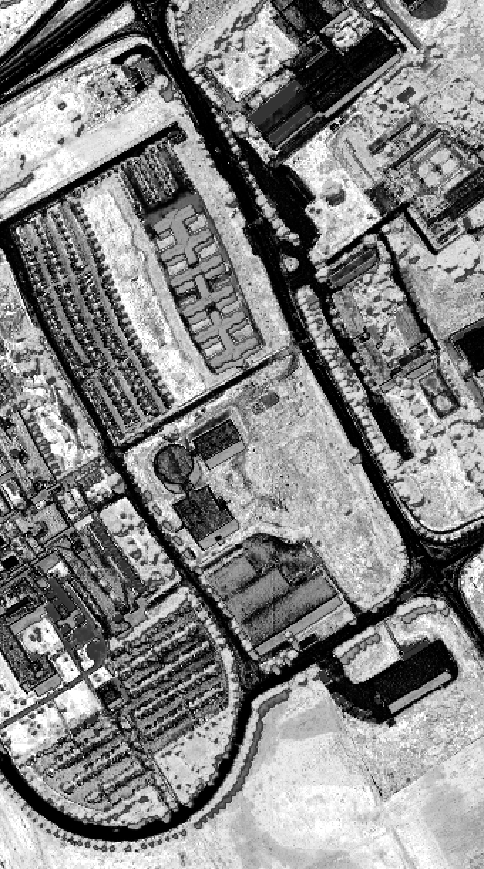
\includegraphics[width=0.9\textwidth]{./figures/proba_uni_1.png}
\end{center}
\end{block}
\end{column}

\begin{column}{0.3\columnwidth}
\begin{block}{Tree}
\begin{center}
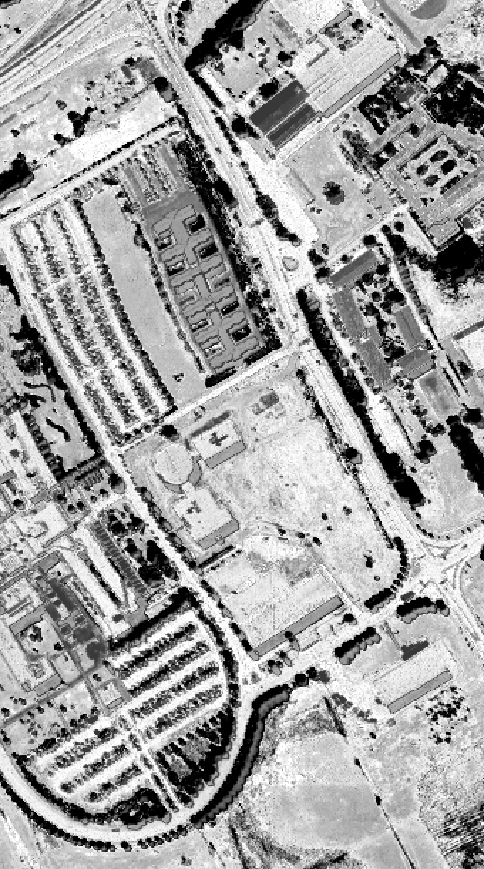
\includegraphics[width=0.9\textwidth]{./figures/proba_uni_4.png}
\end{center}
\end{block}
\end{column}

\begin{column}{0.3\columnwidth}
\begin{block}{Metal sheet}
\begin{center}
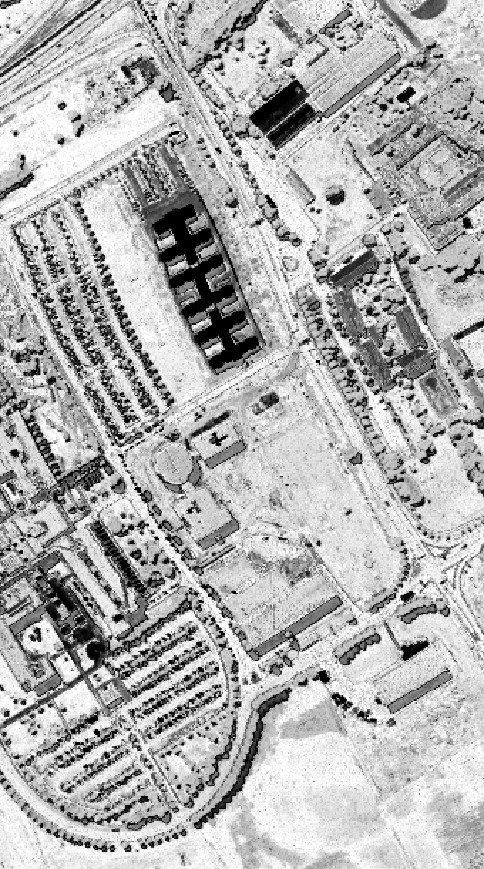
\includegraphics[width=0.9\textwidth]{./figures/proba_uni_5.png}
\end{center}
\end{block}
\end{column}
\end{columns}
\end{frame}

\begin{frame}[label={sec:org6b7a7c4}]{MRF in action 3/3}
\begin{columns}
\begin{column}{0.3\columnwidth}
\begin{block}{Spectral only}
\begin{center}
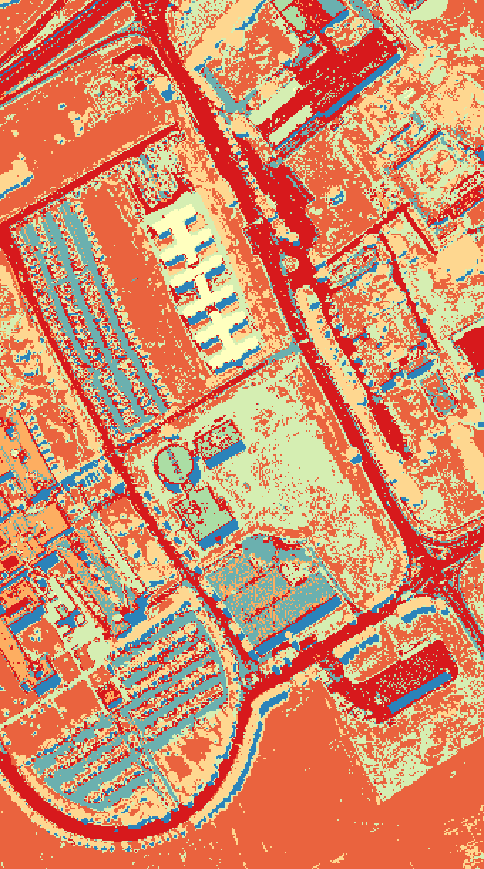
\includegraphics[width=0.9\textwidth]{./figures/mrf_labels.png}
\end{center}
\end{block}
\end{column}

\begin{column}{0.3\columnwidth}
\begin{block}{MRF}
\begin{center}
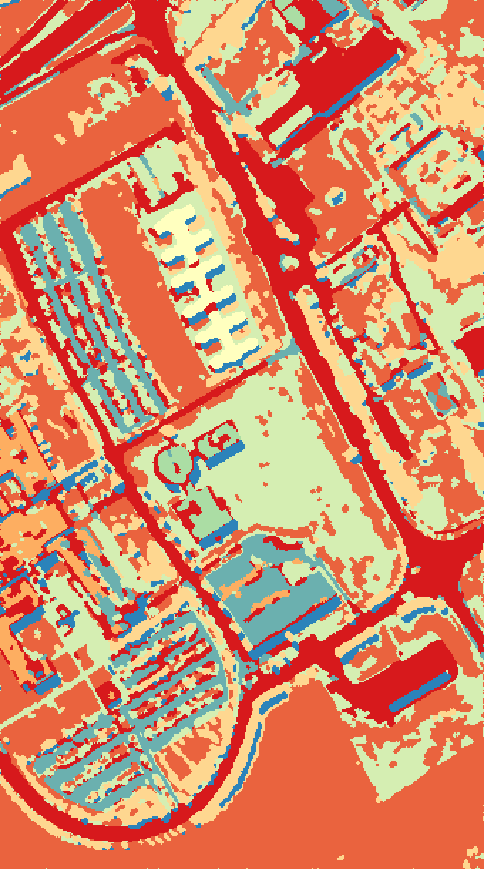
\includegraphics[width=0.9\textwidth]{./figures/mrf_regul.png}
\end{center}
\end{block}
\end{column}

\begin{column}{0.3\columnwidth}
\begin{block}{Iteration}
\begin{center}
  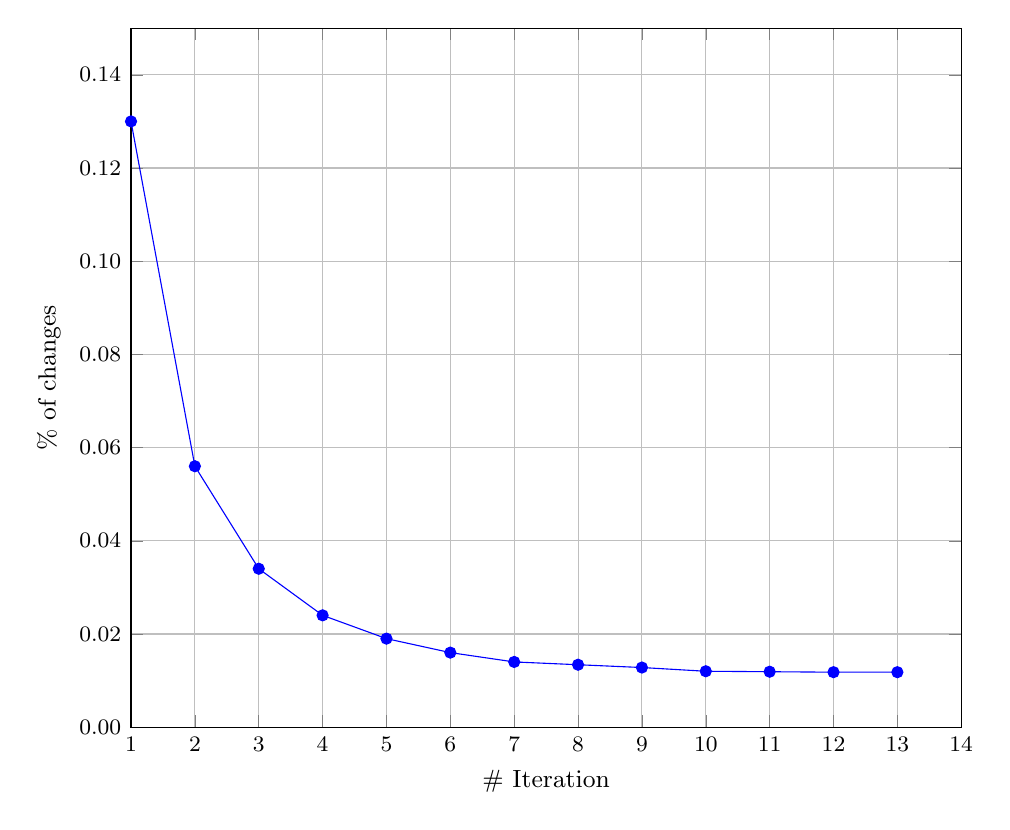
\begin{tikzpicture}
  \begin{axis}[small,width=\textwidth,xlabel=\# Iteration,ylabel=\% of changes,grid=both,xmin=1,xmax=14,ymin=0,ymax=0.15,y tick label style={
        /pgf/number format/.cd,
            fixed,
            fixed zerofill,
            precision=2,
        /tikz/.cd
    },]
    \addplot[blue,mark=*] coordinates {(1,0.13)
      (2,0.056)
      (3,0.034)
      (4,0.024)
      (5,0.019)
      (6,0.016)
      (7,0.014)
      (8,0.0134)
      (9,0.0128)
      (10,0.012)
      (11,0.0119)
      (12,0.0118)
      (13,0.0118)};
  \end{axis}
  \end{tikzpicture}
\end{center}
\end{block}
\end{column}
\end{columns}
\end{frame}

\subsection{Composite kernel}
\label{sec:org630ebfe}
\begin{frame}[label={sec:org22ad08e}]{Operations on kernels}
\begin{itemize}
\item Let \(k_1\)  and \(k_2\) be positive  semi-definite, and \(\lambda_{1,2}>0\) then:
\begin{enumerate}
\item \(\lambda_1k_1\) is a valid kernel
\item \(\lambda_1k_1+\lambda_2k_2\) is positive semi-definite.
\item \(k_1k_2\) is positive semi-definite.
\item \(\exp(k_1)\) is positive semi-definite.
\item \(g(\mathbf{x}_i)g(\mathbf{x}_j)\)  is  positive  semi-definite,  with
\(g:\mathbb{R}^d\to\mathbb{R}\).
\end{enumerate}
\item A kernel  is usually  seen as  a measure  of similarity  between two
samples.  It  reflects in  some sens, how  two samples  are similar.
\item <2> \uline{In  image  classification}. It  is  possible to  build
kernels that includes information from the spatial domain.
\begin{itemize}
\item Local correlation
\item Spatial position
\item Morphological feature,
\item \ldots{}
\end{itemize}
\end{itemize}
\end{frame}
\begin{frame}[label={sec:org58286c6}]{Spatial spectral kernel}
\begin{center}
  \tikzstyle{data} = [draw, ellipse,fill=red!20, node distance=3cm, minimum height=2em]
  \tikzstyle{block} = [rectangle, draw, fill=blue!20,text width=5em, text centered, rounded corners, minimum height=4em]
  \tikzstyle{line} = [draw, -latex']
  \begin{tikzpicture}
    \draw (-3,1) node[data] (spaF) {Spectral Feature};
    \draw (-3,-1) node[data] (speF) {Spatial Feature};
    \draw (2,1) node[block] (k1) {Kernel};
    \draw (2,-1) node[block] (k2) {Kernel};
    \draw (5,0) node[block] (k) {Combination};
    \path [line] (spaF) -- (k1);
    \path [line] (speF) -- (k2);
    \path [line] (k2) -- (k);
    \path [line] (k1) -- (k);
  \end{tikzpicture}
\end{center}

\begin{itemize}
\item From \cite{1576697}:
\begin{itemize}
\item Feature fusion: \(k_{\text{spatial+spectral}}\)
\item Direct summation: \(k_{\text{spatial}} + k_{\text{spectral}}\)
\item Weighted summation: \(\mu k_{\text{spatial}} + (1-\mu)k_{\text{spectral}}\), \(0\leq \mu \leq 1\)
\end{itemize}
\item Can be extended to more than two kernels: \emph{multiple kernel learning} (tricky)
\end{itemize}
\end{frame}
\begin{frame}[fragile,label={sec:org9973fba}]{SS-Kernel in action 1/}
 \begin{itemize}
\item Combination of
\begin{itemize}
\item Spectral bands
\item Spatial features: local median computed on a moving window
\end{itemize}
\item Weighted summation kernel + SVM
\end{itemize}

\begin{minted}[fontsize=\footnotesize,obeytabs=true,tabsize=4,bgcolor=bg]{python}
# Create a pipeline
pipe = Pipeline([
    ('CK',CompositeKernel()),
    ('SVM',SVC())
])

# Optimize parameters
cv_params = dict([
    ('CK__gamma', 2.0**sp.arange(-3,3)),
    ('CK__mu', sp.linspace(0,1,num=11)),
    ('SVM__kernel', ['precomputed']),
    ])
\end{minted}
\end{frame}
\begin{frame}[label={sec:orgfff130f}]{SS-Kernel in action 2/}
\begin{columns}
\begin{column}{0.3\columnwidth}
\begin{block}{Spectral only}
\begin{center}
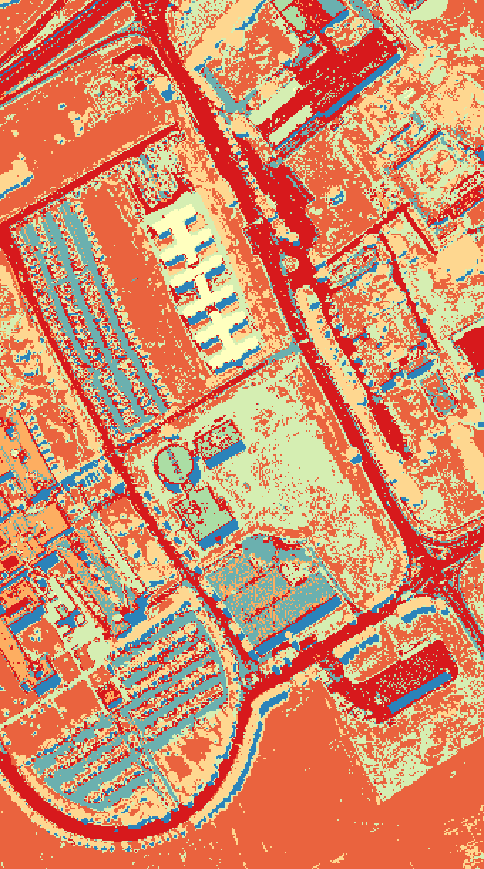
\includegraphics[width=0.9\textwidth]{./figures/mrf_labels.png}
\end{center}
\end{block}
\end{column}

\begin{column}{0.3\columnwidth}
\begin{block}{Composite kernel}
\begin{center}
\includegraphics[width=0.9\textwidth]{./figures/university_tm_ck_mw.png}
\end{center}
\end{block}
\end{column}

\begin{column}{0.3\columnwidth}
\begin{block}{Parameters}
\begin{itemize}
\item F1 = 0.89
\item \(\mu\) = 0.8
\end{itemize}
\end{block}
\end{column}
\end{columns}
\end{frame}

\section{References}
\label{sec:org3281717}
\begin{frame}[fragile,allowframebreaks,label=]{Bibliography}
\printbibliography
\end{frame}
\begin{frame}[label={sec:orgf92bf57}]{}
\begin{center}
\tiny Creative Commons Attribution-ShareAlike 4.0 Unported License
\normalsize

\begin{center}

\includegraphics[width=0.1\textwidth]{figures/cc-by-sa.png}
\end{center}
\end{center}
\end{frame}
\end{document}